\documentclass[11pt]{article}
\RequirePackage{fullpage}
%\RequirePackage[font=small,labelfont=bf]{caption}
\RequirePackage{amsmath,amssymb,amsthm}
\RequirePackage{graphicx}
\RequirePackage[hidelinks]{hyperref}
\RequirePackage{subcaption}
\RequirePackage{wasysym}
\RequirePackage{authblk}
\RequirePackage{bm}
\RequirePackage{bbm}
%\RequirePackage[osf]{mathpazo}
\let\temp\rmdefault
\RequirePackage{mathpazo}
\let\rmdefault\temp

\RequirePackage[bibstyle=authoryear,citestyle=authoryear-comp,
                date=year,
                maxbibnames=9,maxnames=5,maxcitenames=2,
                backend=biber,uniquelist=false,uniquename=false,
                % style=apa,
                sorting=nyt,
                % sorting=,
                hyperref=true]{biblatex}
\usepackage{color}
\usepackage{nicefrac}


% line numbers:
\RequirePackage{lineno}
%\modulolinenumbers[5]
\renewcommand\linenumberfont{\normalfont\tiny\sffamily\color{black}}

\renewcommand{\P}{\mathbb{P}}
\newcommand{\E}{\mathbb{E}}
\newcommand{\V}{\text{V}}
\DeclareMathOperator{\var}{var}
\DeclareMathOperator{\cov}{cov}

\addbibresource{biblio.bib}

\title{Towards a Complete Model of the Negative Selection Process in Humans}

\author{Vince Buffalo and Andrew Kern}

\begin{document}
\maketitle



\begin{abstract} 
% TODO: emphasize connection to nearly neutral theory
\end{abstract}


\section*{Introduction}

The continual influx of new mutations into populations is the ultimate source
of all adaptations, but the vast majority of mutations either do not affect
fitness or are deleterious. Negative selection works to eliminate such
deleterious mutations from the population, which is essential to maintaining
the integrity of information in the genome to maintain a lineage. Mutations
under negative selection are kept at low frequencies (Haldane?), contributing
to human traits (XXX) and diseases. As with most selection in the genome, this
process perturbs the allele frequencies of neighboring linked variation. This
reduces genetic variability around conserved segments and creates large-scale
spatial patterns in genetic diversity. These patterns are mediated by the
deleterious mutation rate, the strength of selection in conserved segments, and
the spatial distribution of recombination rates and conserved segments. Since
genome-wide recombination maps and putatively conserved segments are available
for many species, researchers have combined these with population genetic
theory to estimate the mutation rate and selection coefficients of deleterious
mutations, as well as the overall reduction in genetic variability due to the
negative selection process.

Classic Background Selection (BGS) theory is the predominant model for the
reduction in linked neutral diversity used by statistical approaches to
quantify the impacts of negative selection. However, this model makes some
assumptions for mathematical tractability that could distort inferences about
the negative selection process. First, since fixation probabilities ultimately
depend on the product of the deleterious selection coefficient (s) and
population size (N), the efficacy of negative selection should depend on
demography. Unfortunately, accommodating demography into theoretic negative
selection models remains an open, difficult problem (XXX). Second, building off
classic models of mutation-selection balance (Crow 1970, Kimura and Maruyama
196), the Background Selection (XXX) model assumes that new mutations are
sufficiently deleterious that they are invariably driven to loss. Under this
assumption, the effect of selection is well-approximated by simply rescaling
the neutral coalescent by a reduction factor known as B (XXX). However, this is
only appropriate in a limited domain of parameters relevant to the negative
selection process (XXX). Because the BGS model cannot accommodate the
possibility of fixation for mutations with $Ns \ll 1$, diversity is incorrectly
predicted to fall to zero as the strength of selection diminishes. This weak
selection problem is related to the wider problem of modeling the substitution
rate of deleterious mutation (i.e. the “ratchet” rate). Third, the BGS model
assumes segments under purifying selection are sufficiently far apart that
there is no selective interference between them. This is a matter of degree,
since under sufficiently high mutation rates or with little recombination,
selective interference can occur with a segment. 

In this work, we extend another class of linked selection models that derive
from quantitative genetics to address limitations of the classic BGS model.
These models consider how polygenic fitness variation increases the rate of
stochastic allele frequency change as alleles become randomly linked to fitness
backgrounds. While these models can theoretically accommodate polygenic fitness
variation from any source as long as its rate of change is not too rapid, we
focus specifically on a deleterious-mutations-only model from Santiago and
Caballero (2016). This model is identical to the classic BGS model when
selection against deleterious mutations is strong, but it also correctly
predicts the reduction in diversity and substitutions rates of weakly
deleterious mutations by accurately modeling levels of genic fitness variation.
We extend Santiago and Caballero’s (hereafter the SC16) model so that it can be
used to model genome-wide patterns of diversity under negative selection
processes, and develop Python software to use this theoretic approach to fit
genome-wide models of negative selection. Using forward simulations, we show
this model leads to more accurate DFE estimates under weak selection. While
this new model accommodates the possibility that a given reduction B could be
due to weaker selection, in applying our composite-likelihood method to human
population genomic data, we confirm earlier findings that strong negative
selection at a small fraction of sites fits human data across populations best.
Finally, we show that while this model solves some limitations of the classic
BGS model, simulations reveal another mysterious defect: a poor fit around
$Ns=1$. We show that this can be partially corrected by incorporating the effects
of selective interference on genic variation, but the remaining discrepancy is
due to the build up of negative linkage disequilibrium that cannot be
adequately captured by this model. We find accounting for genic selective
interference between segments fits human population genomic data slightly
better, suggesting levels of negative selection in humans are sufficient to
perturb the selection at other sites.

\section*{Theory}

Our work is motivated by a well-known limitation of classic background
selection theory: it is only accurate for strongly deleterious mutations
\parencite{Charlesworth1993-gb,McVean2000-bt,Good2013-lp,Gordo2002-dr}. Given
statistical methods that fit linked selection processes to genome-wide
diversity data rely on the classic BGS model to estimate the distribution of
fitness effects and rate of deleterious mutations, it is important to
characterize and remedy these shortcomings. However, extending background
selection theory to model weak negative selection is challenging, and it is
worthwhile to develop some intuition for why this is the case, how the classic
background selection works, and how the model of \textcite{Santiago2016-mu}
solves these problems and can be extended to genome-wide inference.

Both the classic background selection and SC16 models imagine a negative
selection process where a continual influx of deleterious mutations flow into
the population at a rate of $\mu$ per basepair per generation in a conserved
region of $L$ basepairs, such that the region-wide per generation mutation rate
is $U = \mu L$. Each mutation imposes an additive selective cost of $s$ in
heterozygotes and $2s$ in homozygotes. The classic background selection model
considers when mutations are sufficiently deleterious that they are destined to
extinction
\parencite{Charlesworth1993-gb,Nordborg1996-nq,Hudson1995-pt,Hudson1994-oh}. In
this case, the genealogy is well-approximated by a neutral coalescence process
with a rescaled effective population size of $N_0 = N \exp(-\nicefrac{U}{s})$.
This approximation works reasonably well for two reasons (though see
\cite{Cvijovic2018-vd,Walczak2012-fi,Nicolaisen2012-vs}). First, when selection
is strong, the number of deleterious mutations per haplotype has a stationary
Poisson distribution with an average equal to the equilibrium under the
deterministic mutation-selection model \parencite{Haldane1927-ga}. Since
lineages carrying any strongly deleterious mutations cannot contribute to the
genealogy, coalescence events only occur in the fraction
$\exp(-\nicefrac{U}{s})$ of the population free of mutations. Second, the time
it takes for a present-day lineage to trace their ancestry back to a
mutation-free ancestor (the ``delay phase") is negligible compared to the
coalescence timescale of $N_0$ among these ancestors (the ``coalescence
phase"), and can be ignored (\cite{Durrett2008-ql}, p. 213;
\cite{Good2014-yz}).

When mutations are only weakly deleterious, their allele frequencies are
strongly influenced by stochastic perturbations and their frequency
trajectories are no longer well-approximated by deterministic models. When
genetic drift is the only source of randomness in allele frequency change, the
relevant scale of stochastic perturbations is determined by the drift-effective
population size $N_e$ (e.g. due to only non-selective process). The insight of
nearly neutral theory (XXX) was that the qualitative behavior of selected sites
is determined by the compound parameter $2N_e s$. When $2N_e s \gg 1$, the
stochastic component of allele frequency change is minuscule relative to
selection and can be ignored; this is why the factor that rescales the
drift-effective population size under the BGS model does not depend on $N_e$.
However, when $2N_e s \le 1$, the stochastic perturbations are on a scale equal
to or greater than the changes due to selection. In this regime, weakly
deleterious alleles can drift up to intermediate frequencies before their
eventual loss or fixation. When this occurs, classic BGS theory breaks down for
several reasons. First, the ``delay phase" is no longer negligible as lineages
carrying weakly deleterious mutations can persist on coalescent timescales.
This distorts genealogies away those expected under neutrality
\parencite{Przeworski1999-mb,OFallon2010-my,Higgs1995-xc}. Second, the
distribution of the number of deleterious mutations (and its corresponding
fitness distribution) are no longer stationary and become a traveling wave
\parencite{Rouzine2008-qz,Good2013-lp,Gessler1995-hz} towards reduced
population fitness (since beneficial mutations are ignored). Consequently,
individuals in the least-loaded class are stochastically lost, fixing those
mutations with a click of ``Muller's ratchet" \parencite{Muller1964-ki}.
Determining both the rate of Muller's ratchet
\parencite{Haigh1978-gt,Gordo2002-dr,Gessler1995-hz} and the shape of
genealogies under weak selection have been stubborn open problems in
evolutionary genetics.

To further complicate matters, both strong and weakly deleterious mutations
create \emph{heritable} fitness variation. In turn, the presence of heritable
fitness variation generates another source of randomness in allele frequency
change known as genetic \emph{draft} \parencite{Neher2013-dz}. An allele
experiences genetic draft when it becomes randomly associated with a fitness
background, which stochastically perturbs its trajectory across generations.
Like genetic drift, perturbations due to draft are directionless but overall
increase the variance in allele frequency change. Unlike drift, stochastic
perturbations caused by draft are autocorrelated across generations for as long
an allele does not recombine or segregate off its fitness background and the
selective environment does not change
\parencite{Robertson1961-ho,Santiago1995-hx,Buffalo2019-qs}. When selection is
strong, draft can generate multiple-merger coalescences that create
discontinuities in allele frequency trajectories, making diffusion
approximations ill-suited \parencite{Gillespie2000-mh,Der2011-it,Neher2013-dz}.
However, when selection is weak, draft can be approximated as an increase in
the rate of drift (or equivalently, a reduction in effective population size).

A key insight from Robertson (\citeyear{Robertson1961-ho}) is that in the
long-run draft acts like an increase in the variance in offspring number.
\textcite{Wright1938-tv} showed that additional non-heritable variance in
offspring number (e.g. due to mating strategy) rescales the population size
according to,

\begin{align}
    \label{eq:simple_Ne}
    N_e = \frac{2N}{V + 2}
\end{align}

However, unlike non-heritable variation in offspring number, the heritable
variation is autocorrelated across generations. At the individual level
Robertson considered, this is because offspring from large families tend to
beget many descendents themselves (and likewise with small families). The same
autocorrelation occurs at the genomic level, as the perturbations to a neutral
allele's trajectory from its particular fitness background tend to occur in the
same direction across generations as long as the linkage exists and the
selective environment is constant. The additional heritable variation in
offspring number is the additive fitness variation $V_A$, which is inflated by
a factor $Q_t^2$ due to the build up of autocorrelation to generation $t$. We
let $Q^2 = Q_t^2$ as $t \to \infty$. Intuitively, the product $V_A Q^2$
represents the expected total variance in reproductive success a neutral
mutation experiences over its lifetime in a system with draft. Incorporating
the impact of time-invariant autocorrelation created by draft as a rescaled
rate of drift is analogous to using the Green--Kubo relation to find the
transport coefficient in molecular dynamics with velocity autocorrelation
\parencite{Green1954-kl,Kubo1957-va}.

Including the total asymptotic variance in reproductive success in Equation
\eqref{eq:simple_Ne} and assuming Wright--Fisher levels of non-heritable
variation (i.e. $V = 2 + 4 Q^2 V_A$), the draft-effective population size $N_d$
is

\begin{align}
    \label{eq:main_Ne}
    N_d = \frac{N}{Q^2 V_A + 1}
\end{align}

(c.f. \cite{Robertson1961-ho,Santiago1995-hx}; see XXX for a proof). In
general, however, statistics such as heterozygosity depend on the cumulative
autocorrelation factor \emph{up to some time} $t$, $Q_t^2$ \parencite[p.
2111]{Santiago1998-bs}. This reflects the fact that effective population size
experienced by a mutation newly associated with a fitness background is larger
than the asymptotic effective population size, since not much autocorrelation
has accumulated in the stochastic perturbations caused by drift yet. From a
backwards-time perspective, this reflects the fact that pairwise diversity
(which is approximately heterozygosity when $2N\mu \ll 1$) depends on the
pairwise coalescence rate per generation, which is not constant under draft.
The benefit of using Robertson's forward-time model of draft is that the
inflation factor is invariant with respect to the particular fitness background
the neutral allele becomes stochastically associated with. By contrast, the
difficulty with modeling draft backwards in time is that the coalescence rates
experienced by a lineage are not invariant to which lineage was sampled due to
its particular associated fitness background.

Equation \eqref{eq:main_Ne} is general, since different modes of selection and
linkage can be accommodated by different expressions for the inflation factor
$Q^2$. When fitness variation has a multiplicative polygenic basis, as it does
for genome-wide negative selection processes, the draft asymptotic effective
population size experienced by an arbitrary neutral site under the influence of
all linked regions is,

\begin{align}
    \label{eq:polygenic_Ne}
    N_d \approx N \exp\left(-\sum_{i=1}^n V_{A,i} \frac{Q_i^2}{2}\right)
\end{align}

where the factor of one-half comes from ignoring weak associations from
unlinked regions and chromosomes (see XXX). In our genome-wide model, we
consider the summation in Equation \eqref{eq:polygenic_Ne} over non-overlapping
segments $i \in \{1, 2, \ldots, n\}$ each undergoing selection such that
segment $i$ contributes additive fitness variance $V_{A,i}$ to the total
additive genetic fitness variance. Under equilibrium levels of fitness
variation, the autocorrelation function for a neutral allele associated with
segment $i$ is the time-invariant function $C(t) = [(1-r_i)(1-\kappa_i)]^t$,
where $r_i$ is the recombination fraction to the segment and $\kappa_i$ is the
rate that the associated fitness variance decays due to selective dynamics.
Then, the cumulative autocorrelation is,

\begin{align}
    Q_i &= 1 + \sum_{j=1}^\infty \left[(1-r_i)(1-\kappa_i)\right]^j \\
        &= \frac{1}{\kappa_i + r_i(1-\kappa_i)}.
\end{align}

(see Appendix Equation \ref{eq:Qinf}). This general equation can accommodate
models of polygenic selection as long as the equilibrium additive fitness
variation $V_{A,i}$ can be specified and the change in variance due to
selection can be approximated as a geometric decay, i.e. $\Delta V_{A,i} =
-\kappa V_{A,i}$ \parencite{Bulmer1971-ae,Keightley1988-eq,Walsh2018-bt}. This
is usually a reasonable assumption since within-generation selection removes a
fraction of phenotypic variation from the population, and some fraction of that
is additive genetic variation \parencite{Bulmer1971-ae,Keightley1988-eq}.

The remaining pieces are expressions for the equilibrium additive fitness
variance $V_A$ and the decay rate in associated fitness $1-\kappa$. At this
point, we diverge from Santiago and Caballero (\citeyear{Santiago1998-bs},
\citeyear{Santiago2016-mu}) to note that the additive fitness variation is the
sum of additive \emph{genic} fitness variance $V_a$ (i.e. due to allele
frequencies) and the total linkage disequilibria $\delta_{LD}$ between selected
sites, $V_A = V_a + \delta_{LD}$. Considering only the genic variation, at
equilibrium $\Delta V_{a,i} = 0$; thus, the loss in genic fitness each
generation due to selective dynamics $-\kappa V_{A,i}$ must be equal to the
increase in fitness variation to new mutations $V_m$ each generation and
changes in the LD term \parencite{Bulmer1971-ae}. Note that the loss in genic
fitness due to drift is not time-invariant due to the build up of
autocorrelation, and considered elsewhere in the derivation (see Supplementary
Materials Equation \ref{eq:vardecay}). Then, $\kappa_i =
\nicefrac{V_{m,i}}{V_{a,i}}$ (see Supplementary Materials Equation \ref{eq:Z}). 

Under any selection model, the genic fitness variance created by a new mutation
(at frequency $x=\nicefrac{1}{2N}$) is $2s^2 x(1-x) \approx \nicefrac{s^2}{N}$.
For the entire population of $2N$ chromosomes, the fresh variance from mutation
each generation in segment $i$ is $V_{m,i} \approx U_is^2$ where $U_i = 2\mu
L_i$ is the diploid mutation rate per generation within the segment. Under
mutation-selection balance assumed by BGS, an $L_i$-basepair segment has genic
variance $V_{a,i}^{BGS} \approx U_i s$ (see Supplementary Materials Equation
\ref{eq:va_bgs}) and thus $\kappa_i^{BGS} = s$. Substituting $V_{a,i}^{BGS}$
and $\kappa_i^{BGS}$ in Equation \eqref{eq:simple_Ne} and simplifying, we have

\begin{align}
    N_d = N \exp \left( - \sum_i^n \frac{\mu L_i}{s(1 + r_i(1-s)/s)^2} \right) 
\end{align}

which is identical to the genome-wide model of background selection used in
previous studies \parencite{McVicker2009-ax,Elyashiv2016-vt,Murphy2022-sj}.
Thus, the classic background selection model is a special case of the more
general theory of Santiago and Caballero (\citeyear{Santiago2016-mu}), which
they have shown previously (\citeyear{Santiago1998-bs}).

When selection is weak, however, the additive fitness variance under the
classic BGS model is no longer accurate. \parencite{Santiago2016-mu} suggested
that this is due to the loss of fitness variation that occurs when a
segregating site fixes and its heterozygosity becomes zero. If we let $R$
represent the rate of the ratchet of deleterious mutations in fixations per
generation, each fixation removes the equivalent amount of equilibrium
variation put in by mutation. Thus, the steady-state genic variance under
mutation and negative selection is (omitting the segment index $i$ for
clarity),

\begin{align}
  \label{eq:Va}
  V_{a} = (U - 2 R)s. 
\end{align}

where the condition $V_a \ge 0$ is met when the probability of fixation is less
than or equal to the neutral fixation probability of $\nicefrac{1}{2N}$, which
is held when considering deleterious mutations. This equation connects the
equilibrium additive genic fitness variance to the flux of new variation in due
to new deleterious mutations and the flux out due to their substitution and the
decline in mean population fitness. When $R=0$, the selection is so strong it
cannot fix, and the equilibrium fitness variation is due entirely to young rare
mutations before their extinction $V_a = V_a^{BGS} = Us$. Santiago and
Caballero demonstrate Equation \eqref{eq:Va} through Fisher's Fundamental
Theorem of Natural Selection, but we find an alternative proof
(\cite{Higgs1995-xc}; see Supplementary Materials Section
\ref{supp:weak-strong}). We find that the steady-state additive genic variance
in Equation \eqref{eq:Va} also results from diffusion models with a flux of
mutations into discrete sites (\cite{Kimura1969-jw}; see Supplementary
Materials Section \ref{supp:kimura}). Our results differ from
\parencite{Santiago2016-mu}, since we find from simulations their expression
models the additive \emph{genic} fitness variation, not additive genetic
fitness variation (see Section XXX). This is because Equation \eqref{eq:Va}
does not capture the expected build-up of negative linkage disequilibria when
selection is only mildly deleterious.

While using Equation \eqref{eq:Va} in Equation \eqref{eq:main_Ne} leads to a
prediction for the draft-effective population size $N_d$, closed-form
expressions for the rate of the ratchet $R$ have generally been hard to find
\parencite{Haigh1978-gt,Higgs1995-xc,Gessler1995-hz}. The key insight of
\textcite{Santiago2016-mu} is that the ratchet rate under draft is determined
by the probability of fixation $p_f(N_d, s)$
\parencite{Kimura1962-su,Malecot1948-zv} with the draft-rescaled effective
population size, e.g. $R = N U p_f(N_d, s)$. Given this equation for the
ratchet and Equation \eqref{eq:polygenic_Ne} for $N_d$ under draft, we have a
system of two non-linear equations that can be solved numerically for $N_d$ and
$R$ for each segment,

\begin{align}
  \label{eq:main_eqns}
  N_d &= N \exp \left( -V_a \frac{Q^2}{2} \right) & \text{\emph{draft-effective population equation}} \\
  R &= \frac{4N_d U s}{\exp(4 N_d s)-1}  & \text{\emph{ratchet equation}}
\end{align}

where $V_a = (U-R)s$ as in Equation \eqref{eq:Va}.

% where,

% \begin{align}
%   V_a &= (U - R(x)) s & \text{\emph{fitness variance equation}} \\
%   Q^2 &= \frac{2}{(1-Z)(2-(2-M)Z)} & \text{\emph{linkage inflation factor}} \\
%   Z &= 1 - \frac{Us}{U-{R(x)}} & \text{\emph{}} \text{\emph{variance decay rate}}
% \end{align}



\section*{Results}

Similar to previous work, our method characterizes the negative selection
process through the signal left on pairwise diversity at linked sites. Although
pairwise diversity is a less-informative statistic than the full site frequency
spectrum, it is much easier to derive models of how selection alters expected
pairwise coalescence times at linked sites than to describe the entire
genealogy. Spatial patterns of pairwise diversity are highly variable across
eukaryotic genomes, as linked selection leads diversity to become correlated
with spatial heterogeneity in recombination rates and the density of conserved
sites. Statistical methods then fit observed diversity to the expected level
under a particular theoretic model of linked selection processes. Consequently,
statistical inferences about selection may be incorrect when the underlying
theory inaccurately predicts average pairwise coalescence times.

\subsection*{Simulations of a Segment under Negative Selection}

\begin{figure}[htbp] \centering
    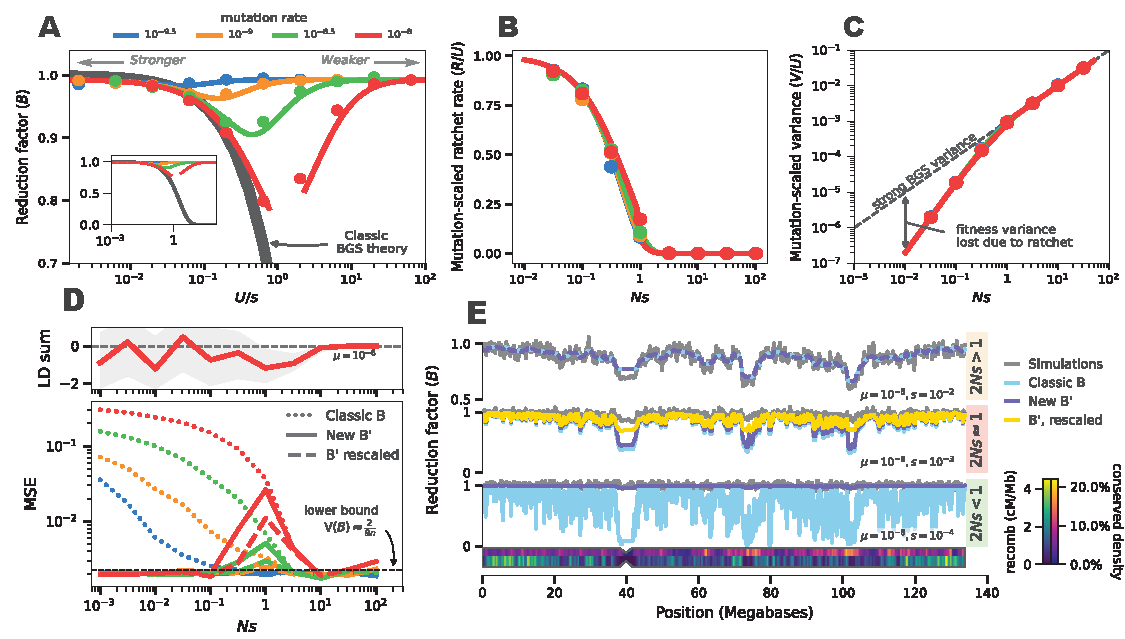
\includegraphics[width=\textwidth]{figures/figure_1.pdf} \caption{Theory
        compared to simulation results. (A) The predicted reduction factor
        under classic B theory (dark gray line) and the diploid SC16 model
        (colored lines corresponding to mutation rate) compared to average
        reduction across XXX simulation replicates (points). (B) The predicted
        ratchet rate under the SC16 model scaled by mutation rate (colored
        lines) compared to the ratchet estimated from simulation (points). When
        $2Ns>1$, the ratchet rate is near zero. (C) The genic variance from
        simulations (points) against the predicted variance under the SC16
        model (colored lines). As the ratchet begins to click, the genic
        variance is decreased from the level expected under strong BGS (dashed
        line). (D, bottom) The mean squared error (MSE) between
        whole-chromosome simulations and predicted classic B (dots), new B'
        (solid), and locally-rescaled B' (dashed) for different mutation rates
        (colors). The dashed horizontal line is the approximate theoretic
        minimum MSE. (D, top) The build up of negative linkage disequilibria
        around $2Ns=1$ in whole-chromosome simulations in bottom panel. (E) The
        average B map from 100 chromosome 10 simulation replicates (gray)
    against different predictions, for parameters that correspond to $2Ns < 1$,
$2Ns = 1$, and $2Ns > 1$. The chromosome shows the density of conserved sites
and recombination map used in simulations. }
  \label{fig:figure-1}
\end{figure}

Given that Santiago and Caballero's (\citeyear{Santiago2016-mu}) model is a
haploid-model for a single region under equilibrium negative selection, we
first sought to confirm it could accurately predict the reduction in realistic
forward-time simulations of diploid populations with recombination. Using SLiM
\parencite{Haller2019-vu,Haller2023-uk} we simulated a region of $10^5$
basepairs under varying levels of mutation and selection. We find a close
correspondence between the observed and predicted reduction in effective
population size $B=\nicefrac{N_d}{N}$ over all selection and mutation
parameters including weak selection (Figure \ref{fig:figure-1}A), in contrast
to classic BGS theory. Furthermore, to investigate whether this accuracy was
caused by the model capturing the equilibrium fitness variance and ratchet
rate, we also measured these throughout the simulation. Again, we find the
diploid SC16 theory accurately predicts both the ratchet rate (Figure
1\ref{fig:figure-1}B) and the genic fitness variance (Figure
1\ref{fig:figure-1}C).

Additionally, these figures provide further intuition for the underlying
negative selection process. When selection is strong the ratchet rate is zero,
as there is no probability that strongly deleterious can fix. However, around
$2N_e s \approx 1$, the ratchet begins clicking as $p_F > 0$. Ultimately, the
ratchet rate reaches the neutral mutation rate, as $V_a = 0$ and $N_d = N$
(e.g. no draft). Likewise, the additive genic fitness variance matches the
level predicted by BGS ($Us$), but begins to diverge when the ratchet begins
clicking. This occurs when the level of variation diverges from the
deterministic mutation-selection equilibrium $V_a = Us$ due to the stochastic
clicking of the ratchet at rate $R$.

\subsection*{Chromosome-wide Simulations and Models of Negative Selection}

Given the accuracy of the SC16 model in predicting the reduction in effective
population size and ratchet rate when equilibrium negative selection processes
were acting in single segment, we extended their model so that it could be
applied to whole-genome data. Our method, implemented in the software
\texttt{bgspy}, calculates the equilibrium additive genic fitness variance
$V_a$ and ratchet rate $R$ for each specified segment in the genome for a range
of mutation rates and selection coefficients and a fixed genome-wide
drift-effective population size $N$ (see Methods XXX). Genomic regions
putatively under negative selection (e.g. coding sequences or UTRs) and the
recombination rate map are specified as arguments so that the predicted values
accurately reflect local genomic details. Note that each equation is solved
independently, since here we assume no selective interference between segments.
We refer to the prediction reductions along the genome from our approach as B'
maps (analogous to B maps from \cite{McVicker2009-ax}).

To assess our B' maps, we simulated negative selection for fixed mutation rates
and selection coefficient on human chromosome 10 using realistic recombination
and conserved feature maps. Averaging over $n=100$ simulation replicates, we
estimated the simulation expected reduction map and compared this to the
predicted B and B' maps for the same parameters. We find that our B' maps and
the classic BGS theory B maps closely match simulations when selection is
strong (top row of Figure \ref{fig:figure-1}E). This provides the first
realistic forward-time simulation confirmation of classic background selection
theory. However, we find slight discrepancies in regions with low recombination
(Figure \ref{fig:figure-1}E). Second, we find our theory is vastly more
accurate than the classic B maps when selection is very weak ($2N_e s \ll 1$;
bottom row of Figure \ref{fig:figure-1}E), which is expected since BGS theory
does not work in this domain. Across all mutation and selection parameters
simulated, the relative error of the classic B maps is 14.6\% whereas the
relative error in the new B' maps is 5\%. Additionally, we find that the mean
squared error between simulations and B' maps is close to the theoretic lower
bound set by the coalescence variance \parencite[see Methods
XXX]{Tajima1983-gu}.

Nearly all of the error between the new B' maps and chromosome-wide simulations
occurs around the drift-barrier domain of $2Ns \approx 1$ (Figure
\ref{fig:figure-1}D). The higher error in this domain occurs across all
mutation rates. First, we hypothesized that the reason this occurred was the
when we numerically solve Equations \eqref{eq:main_eqns} for each segment, this
does does not consider the reduction due to selection at other linked segments.
In particular, we use $N=1000$ corresponding to the number of diploids in the
simulations rather than $B'(x) N$ at position $x$. To test this, we implemented
a locally-rescaled version of the B' maps, which numerically solves Equations
\eqref{eq:main_eqns} for each segment at position $x$ taking into account the
reduction experienced due to selection at other segments by setting $B'(x)N$ as
the population size (see Method XXX). We find the locally-rescaled B' maps
reduce the relative error from 5\% to 0.4\% and mean squared error (Figure
\ref{fig:figure-1}D, dashed colored lines), but does not entirely eliminate the
error in the $2Ns \approx 1$ domain.

Finally, we hypothesized that the remaining error is because of the build up of
negative linkage disequilibria between selected sites due to Hill--Robertson
interference \parencite{Hill1966-kd,McVean2000-bt,Comeron2007-wq}. To assess
this possibility, we calculated the sum of all linkage disequilibria in our
chromosome-wide simulations. We find negative linkage disequilibria build ups
around $2Ns \approx 1$ (Figure \ref{fig:figure-1}D, top row) and is stronger
when mutation rates are higher (Supplementary Figure XXX). As $Ns \to 0$, the
variance in LD inflates as expected \parencite{Ohta1969-ae,Hill1968-ue}.
Overall, the build up of negative LD is consistent our view that the
equilibrium fitness variance modeled by the SC16 theory is the additive
\emph{genic} fitness variance, which differs from the additive genetic variance
by the sum of linkage disequilibria between selected sites (i.e. $\delta_{LD} =
s^2 \sum_{i\ne j} D_{i,j}$ where $D_{i,j}$ is the LD between sites $i$ and
$j$). However, according to theory, the reductions in diversity should be
determined by levels of additive genetic fitness variance that include the
contribution of LD (Supplementary Materials Section XXX).

\subsection*{Annotation Model Comparison}

Our method takes tracks of annotated features that are \emph{a priori} expected
to have similar fitness effects, and estimates the distribution of fitness
effects for each feature type. Additionally, our method estimates the
per-basepair per-generation deleterious mutation rate ($\mu_\text{del}$) and
the background level of pairwise diversity ($\pi_0$). Since the theory used by
our method can in principle accommodate weak selection and neutrality. To test
this, for each our annotation models, we fit (1) ``sparse" models that only
cover the fraction of the genome that is the union of all tracks, and (2)
``full`` models that are sparse models with the remaining complement of the
genome labeled as ``other".

Overall, we find that 

\begin{figure}[htbp] \centering
    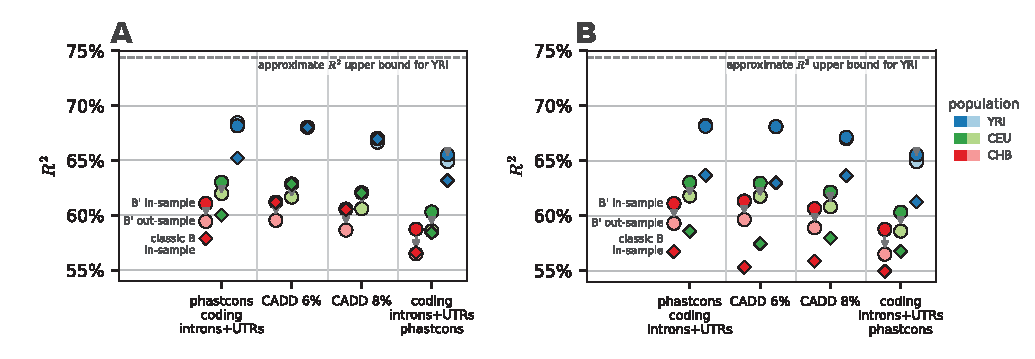
\includegraphics[width=\textwidth]{figures/figure_2.pdf} 
    \caption{The $R^2$ estimates for a sparse (A) and full (B) models, for all 
    populations (colors). Round points are our B' method; diamonds are the 
    classic B. For our method, we also calculate leave-one-out out-sample $R^2$
    (lighter filled points).}
  \label{fig:figure-2}
\end{figure}

\subsection*{Estimates of Negative Selection in Humans}

\begin{figure}[htbp] \centering
    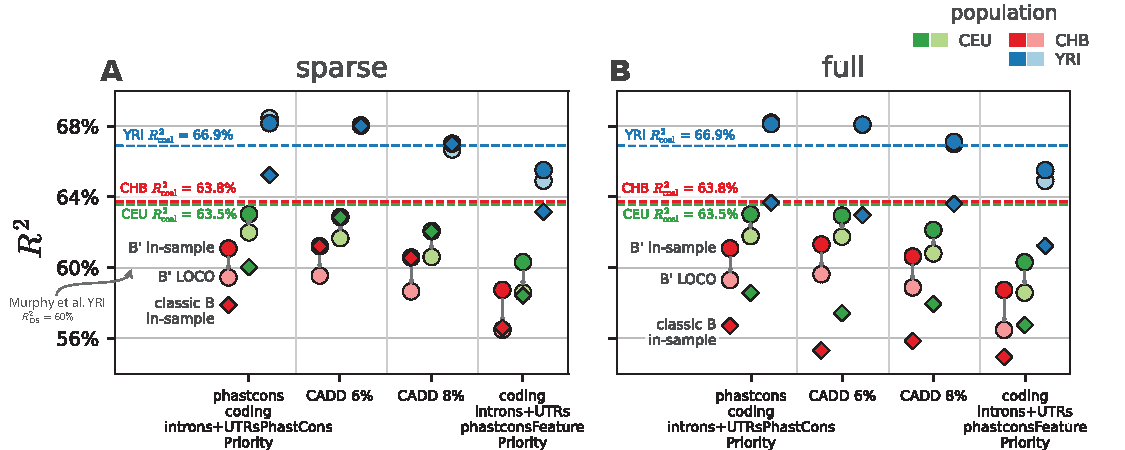
\includegraphics[width=\textwidth]{figures/figure_3.pdf} 
    \caption{The distribution of fitness effects of new mutations estimates for
        Yoruba individuals. (A) The DFEs using sparse (left column) and
        full-coverage (right column) tracks, across different annotation models
        (row). Color indicates the feature type. (B) The DFE of the
        full-coverage CDS-priority model comparing the estimates across
    populations.}
  \label{fig:figure-3}
\end{figure}



Next, we developed a composite-likelihood method to estimate pairwise diversity
in the absence of linked selection $\pi_0$, the deleterious mutation rate
($\mu_D$), and distribution of fitness effects ($\mathbf{W}$) under negative
selection. Because the focus of our work is to fix deficiencies in the classic
BGS model, our current implementation does not consider reductions in diversity
due to recurrent hitchhiking or other positive selection processes. Since
previous work has established that purifying selection is the dominant mode of
linked selection in humans and hitchhiking plays a limited role
\parencite{McVicker2009-ax,Murphy2022-sj}, humans are a suitable organism to
test our method. 

Given that previous methods used classic BGS theory to fit genome-wide patterns
of human diversity, we were curious whether their qualitative findings would
change once weak selection was more accurately predicted. In particular, the
U-shaped relationship between $B'$ and the strength of selection suggests that
a given reduction factor could be explained by two different selection
coefficients.

\subsection*{DFE Estimates}

\begin{table}
\centering
\caption{$R^2$ and mutation rate estimates for all models}
\begin{tabular}{lll|crr|cc}
    \textbf{Model} & \textbf{Track type} & \textbf{Pop.} & \textbf{B' $R_\text{LOO}^2$} & \textbf{B' $R_\text{IS}^2$} & \textbf{B $R_\text{IS}^2$} & \textbf{B' $\hat{\mu} \times 10^{-8}$} & \textbf{B $\hat{\mu} \times 10^{-8}$} \\[0.5ex] 
\hline
\hline
    \textbf{phastcons$>$CDS$>$genes} &            sparse &          YRI &                        \textbf{68.45} &             68.16 &            65.23 &                                 1.8636 &                                0.2975 \\
phastcons$>$CDS$>$genes &              full &          YRI &                        68.19 &             68.12 &            63.67 &                                 1.7082 &                                0.1666 \\
               CADD 6\% &              full &          YRI &                        68.08 &             68.08 &            62.96 &                                 1.4612 &                                0.1721 \\
               CADD 6\% &            sparse &          YRI &                        68.04 &             68.03 &            68.01 &                                 2.0912 &                                2.0716 \\
               CADD 8\% &              full &          YRI &                        66.98 &             67.11 &            63.61 &                                 1.0126 &                                0.1713 \\
               CADD 8\% &            sparse &          YRI &                        66.67 &             67.01 &            66.98 &                                 1.5688 &                                1.5473 \\
CDS$>$genes$>$phastcons &              full &          YRI &                        64.90 &             65.51 &            61.23 &                                 4.1951 &                                0.1620 \\
CDS$>$genes$>$phastcons &            sparse &          YRI &                        64.90 &             65.51 &            63.16 &                                 4.1795 &                                0.3070 \\
\textbf{phastcons$>$CDS$>$genes} &            sparse &          CEU &                        \textbf{61.98} &             63.02 &            60.02 &                                 2.0194 &                                0.3036 \\
phastcons$>$CDS$>$genes &              full &          CEU &                        61.78 &             63.01 &            58.57 &                                 2.3499 &                                0.1679 \\
               CADD 6\% &              full &          CEU &                        61.74 &             62.94 &            57.42 &                                 1.5365 &                                0.1739 \\
               CADD 6\% &            sparse &          CEU &                        61.66 &             62.86 &            62.84 &                                 2.1215 &                                2.1084 \\
               CADD 8\% &              full &          CEU &                        60.80 &             62.12 &            57.95 &                                 1.1572 &                                0.1742 \\
               CADD 8\% &            sparse &          CEU &                        60.59 &             62.06 &            62.04 &                                 1.6030 &                                1.5876 \\
               CADD 6\% &              full &          CHB &                        59.62 &             61.31 &            55.31 &                                 1.5083 &                                0.1727 \\
               CADD 6\% &            sparse &          CHB &                        59.54 &             61.21 &            61.20 &                                 2.1242 &                                2.1170 \\
               \textbf{phastcons$>$CDS$>$genes} &            sparse &          CHB &                        \textbf{59.44} &             61.08 &            57.88 &                                 2.1982 &                                0.3060 \\
phastcons$>$CDS$>$genes &              full &          CHB &                        59.29 &             61.08 &            56.71 &                                 2.5573 &                                0.1694 \\
               CADD 8\% &              full &          CHB &                        58.88 &             60.63 &            55.86 &                                 1.1128 &                                0.1733 \\
               CADD 8\% &            sparse &          CHB &                        58.65 &             60.57 &            60.55 &                                 1.6098 &                                1.6001 \\
CDS$>$genes$>$phastcons &            sparse &          CEU &                        58.58 &             60.30 &            58.41 &                                 4.1041 &                                0.3110 \\
CDS$>$genes$>$phastcons &              full &          CEU &                        58.58 &             60.30 &            56.75 &                                 4.1001 &                                0.1648 \\
CDS$>$genes$>$phastcons &            sparse &          CHB &                        56.48 &             58.73 &            56.60 &                                 3.7195 &                                0.3136 \\
CDS$>$genes$>$phastcons &              full &          CHB &                        56.48 &             58.73 &            54.95 &                                 3.7552 &                                0.1654 \\
\hline
\end{tabular}
\end{table}

Our best-fitting models have out-sample $R^2$ of around 68\% for Yoruba, 62\%
European, and 60\% for Han Chinese ancestry individuals. However, $R^2$ has a
theoretic upper bound due to coalescence noise around the predicted mean level
$\widehat{\pi}(x)$.



% - Table s5 https://oup.silverchair-cdn.com/oup/backfile/Content_public/Journal/genetics/206/1/10.1534_genetics.116.197145/8/files1.pdf?Expires=1686357613&Signature=cp9qoI2ChCb6GFZ74HI4eWcA~MQ4sHlWyeI3Zp49-5xEORzMfYlSRxzVvZlo8ZoGWDi0G3PnL00ZplM-~or4YIVm2uhkmqjf61AmC7RdZ1QTak4j0kFMQ0wAbM9pusiV3gIepTQHq2HKRKwgS~ypmv~0oqO5dDxaq9nhOWIBBmLAA49oHWuxUtnRe3sEYATwCwjIFEomhgJpg7vKGCF~87GdCV4JETW4PN2VvD4hsu2AVRd8yA~vUJvsXfhWwcElDeY4fsgpprl1lC3XGjJCnqdwbzRGPV5LNx5XEKLptcZtLeLcOmFJCvmVLe0bewJ7Vta0TSQM7T9AuklompjPPw__&Key-Pair-Id=APKAIE5G5CRDK6RD3PGA

Like other methods, our method divides the putatively conserved basepairs up

Generally, when the putatively conserved region is larger, there is a tradeoff
in two dimensions. First, more bases are conserved according to the same DFE,
so the total mutational load increases. This causes the tradeoff between
mutation rate estimate and CADD fraction we observe across both our B' model
and the classic B when using sparse tracks (Figure 2XXX). 


We find that mutation rate estimates are fairly sensitive to model choice
(Figure 2XXX). 

Since B' has a U-shaped relationship with the selection coefficient, we
hypothesized that our model may reveal true identifiability issues in
estimating the DFE that do not occur under the classic B model. We find that
this is not the case for our models fit at the megabase-scale. The DFE
estimates for our CADD6 and CADD8 models are consistent (Figure XXX), and both
produce similar mutation rates.

While we do not comprehensively fit all of our model to other spatial scales,
we 

However, while a given reduction level may be explained by either a weak or
strong selection coefficient, the spatial extent of these reductions caused by
weak selection is much narrower than under strong selection. 

We see evidence this is the case in several of our models, where
genome-wide diversity fits equally well between models with mutation rates 

Indeed, we see this by comparing parameter estimates of the CADD6
sparse-track model using classic BGS B and our B' method. 


(which mimics the best-fitting model of
\cite{Murphy2022-sj}) 

(see also
Appendix 1, Figure 26A of \cite{Murphy2022-sj})

correlation between s and feature

Overall, we find evidence that negative selection models are very sensitive to
the input track. Because inference based on our B' method accommodates weaker
selection, the primary models we fit here more robust to misspecification of
the regions

\subsection*{Evolutionary Models}

We model the diversity at punitively neutral sites. These are sites in regions
we have \emph{a prior} reason to believe have a DFE nearly entirely
concentrated in the neutral range. While this may not be the case in reality,
it is necessary given the computational demands of modeling whole-genome
selection. 

CDS+phastcons+UTR model

 - UTR as neutral control

 - CDS takes priority over phastcons, phastcons is fallback. Otherwise, the
   effect of CDS would be biased by the fraction removed and classified as
   phastcons. This is the right comparison for the substitution model.

\subsection*{Predicted Substitution Rates}

- mention neg. auto correlation?

- Gene level analysis

To evaluate the predicted substitution rate of our CDS+phastcons+UTR model, 


Additionally, our GBGS model makes predictions about the rate of substitutions
in different segments under purifying selection. There are two stages of the
prediction process. First, when the initial B' maps are calculated, the
predicted substitution rate is calculated as a byproduct of 

\section*{Discussion}

It is worth considering why this model performs well for models of negative
selection. The fitness variance equation, $V(x) = (U-2R)s$ tells us that under
models, the long-run variance is set by the balance of mutation and fixation.
Whether a particular basepair's behavior follows this equation depends upon
whether the long-run average is close to ``typical" for that basepair at a
given time. Good things fix so quickly, that we're left with a constant
churning of new variation

- need for coalescent simulations with reduced $N_e$ along the genome.

- we need to talk about Fisher's Fundamental Theorem and how this model
connects fitness variation to absolute changes in fitness.


\section*{Methods}


\subsection*{Chromosome-wide Simulations}

, using the HapMap recombination map (XXX) and in coding regions, PhastCons
regions, and UTRs as an approximate set of putatively conserved segments

We calculate the mean squared error (MSE) and relative error between
whole-chromosome simulations and the predicted B and B' maps by averaging
branch diversity in 10 kilobase windows (tskit, XXX) and dividing by the
neutral expectation of $4N$. The theoretic lower bound of the MSE is due the
noise in estimating the expected reduction map from simulations. For $n=100$
replicates, the sampling noise is minimal relative to the evolutionary noise in
the coalescence process \parencite{Tajima1983-gu}. We use this as the theoretic
lower bound assuming the maximum coalescence noise at $B=1$, $\var(\bar{B})
\approx \nicefrac{2}{9n}$.


\subsection*{Local-rescaled }
We note that it is computationally intractable to solve this equation excluding
the contribution of the focal segment 



\subsection*{Solving the B' Equations for each Segment}

In our implementation of the theory of \textcite{Santiago2016-mu}, we calculate
the local effective population size $N_e(x) = b(x) N$ within a segment $x$ by
solving a system of two non-linear equations, 

\begin{align}
  \label{eq:}
  {N}_{e}(x) &= N \exp \left( -\frac{V(x)}{2} Q^2(x) \right) & \text{\emph{effective population equation}} \\
  {R}(x) &= \frac{4N_e(x)U s}{\exp(4 N_e(x) s)-1}  & \text{\emph{substitution equation}} 
\end{align}

where,

\begin{align}
  %V(x) &= U s - 2 {R}(x) s & \text{\emph{fitness variance equation}} \\
  V(x) &= (U  - 2 {R}(x)) s & \text{\emph{fitness variance equation}} \\
  Q^2(x) &= \frac{2}{(1-Z)(2-(2-M)Z)} & \text{\emph{linkage inflation factor}} \\
  Z &= 1 - \frac{Us}{U-{R(x)}} & \text{\emph{}} \text{\emph{variance decay rate}}
\end{align}

and $U = \mu L$ and $M = r_\text{BP} L$ are the total mutation and
recombination rates for a segment $L$ basepairs long. Each mutation has a
selection coefficient of $s$, for which we assume additive effects. Then, the
local reduction factor is $b(x) = \nicefrac{N_e(x)}{N}$, and the per-basepair
per-generation substitution rate is $\lambda_D = \nicefrac{R(x)}{L}$. Note that
in the variance equation, the long-run variance is the balance between mutation
and twice the loss due to substitution, $(U-2R)s$, since for selective balance
$V(x) = 0$ for $s>0$, the per-basepair substitution rate must be half the mutation rate,
since each substitution removes twice the variance introduced by a mutation in
a diploid species.

In our software \texttt{bgspy}, these two equations are solved for a grid of
mutation rates and selection coefficients for each specified segment from a
feature type (e.g. CDS, UTRs, etc.). This results in estimates of $N_e(x)$ and
$R(x)$ per segment. In the first-round B' calculation, we use a single
pre-specified drift-effective population size, $N$. The B' maps created here at
this step reflect selection only in the segment, ignoring the impact of
selection at other segments. By contrast, the locally-rescaled B' maps solve
these equations, assuming the drift-effective population size is $B(x)N$. These
reflect the segment's dynamics if they were effected by selection at other
segments under selection in the genome. Consequently, we can compare and
contrast models with local-recalling to test whether we achieve a better fit if
we account selective interference from other segments.

\subsection*{The B' Maps}

The reduction at a focal site $x$ can be calculated as the product of all
segments' contributing reduction factors, 

\begin{align}
  B(v) = \prod_x b(x,v)
\end{align}

where $b(x, v)$ is a modified version of $b(x)$ that accounts for the
recombination between the segment $x$ and the neutral site $v$ (see XXX).

In practice, we calculate B' using the variables determined by solving the B'
equations for each mutation and selection coefficient in the grids. Since only
the analog of $Q^2(x)$, $Q^2(x, v)$ changes, the pre-computed substitution rate
(and thus local variance) can be re-used for each $v$. We calculate $B(v)$
across a grid of focal points along the chromosome, spaced 10kb apart.

\subsection*{Assessing the B' Maps}

We first assessed the B' maps against the observed average reduction across
$XXX$ forward-simulations, $\bar{B}_\text{sim}(x)$. The mean-squared error has
two sources, (1) bias from a breakdown in our theory $B(x)$ for the average
reduction, and (2) variance from the simulations. We show that for most of the
parameter space, the measured mean-squared error between simulation averages
and our B' maps is at the theoretic minimum. This minimum variance is entirely
from the coalescent noise when estimating $\bar{B}\text{sim}(x)$, which 

\subsection*{Maximum Likelihood Estimation}

\subsection*{Local Rescaling and Substitution Rate Prediction}


\subsection*{Substitution Rate Predictions}

Our MLE fit $\hat{\Phi}$ also implies a set of corresponding substitution rate
predictions for each segment under mutation-selection-draft process. There are
two sources of variation in these predictions in this model. First, there is
the variation across the pre-specified functional categories, e.g. CDS, UTRs,
and PhastCons. Second, there is region-specific variation 









% As genomes are transmitted through the generations, lifetime events selectively
% alter what is passed to the next generation. While selection directly acts on
% the genetic variants that cause heritable fitness differences among
% individuals, neighboring regions experience an indirect contraction in genetic
% variability. This byproduct is known as \emph{linked selection}, and it occurs
% when selection changes a site's frequency on timescale faster than
% recombination can decouple that site from its genetic background. Because
% linked selection modifies the genetic variability in a regionally-correlated
% way, it creates observable patterns in genomic data that are used to understand
% the type of selection processes acting on genomes and estimate key evolutionary
% quantities. 

% , with characteristic length
% $\nicefrac{s}{r}$ basepairs, where $s$ is the heterozygous selection
% coefficient and $r$ is the per-basepair recombination rate. Sweeps were found
% in humans, \emph{Drosophila}, and other species (XXX), though it was unclear
% whether hitchhiking alone could explain the observed genome-wide correlation
% between recombination rate and genetic diversity in some species (XXX). 

% Much work has been done on developing mathematical theory for two linked
% selection processes: hitchhiking and background selection. These are
% distinguished by the evolutionary processes that generate fitness variation and
% the resulting selection dynamics. Under the classic hitchhiking model, a new
% beneficial mutation sweeps fixation, leading to a dip in genetic diversity on a
% small spatial scale. Since the sweeps leave relatively narrow footprint, they
% influence genome-wide diversity only when beneficial mutations are recurring
% and recombination is relatively limited, as in \emph{Drosophila}. These models
% assume sweeps are sufficiently rare as to not occur simultaneously, which is
% consistent with the slow estimated rate of strongly beneficial mutations (XXX).
% Overall, the classic hitchhiking model is simple because the underlying
% selection process does not generate polygenic fitness variation, even though
% this is type of variation plays a dominant role in adaptation (XXX).

% By contrast, background selection is a consequence of the fitness variation
% created by a steady influx of new deleterious mutations. The classic background
% selection model (XXX) considers how the balance between mutation introducing
% deleterious variants into the population and selection removing them, reduces
% nearby genetic variability. A critical assumption of this model is that such an
% equilibrium between mutation and selection exists, which is the case only when
% these mutations have a large enough fitness cost to ensure that they cannot fix
% in the population. Under this process, the number of deleterious mutations per
% gamete reaches a Poisson stationary distribution with rate $\nicefrac{U}{s}$,
% where $U = \mu_D L$ is the deleterious mutation rate ($\mu_D$ per basepair per
% generation) in a region of $L$ basepairs for mutations with a heterozygous
% selection coefficient of $s$ (XXX). The fraction of gametes without any
% mutations is then $f_0 = \exp(-\nicefrac{\mu_D}{s})$. Without recombination,
% any gamete with deleterious mutations is destined to bring its linked neutral
% variation with it to extinction, effectively reducing diversity levels to those
% expected in a neutrally-evolving population of size $f_0 N$. 

% Remarkably, predictions from simple background selection models with
% recombination closely match large-scale patterns of human diversity and
% divergence (XXX). Since background approximately rescales a neutral coalescent
% process by $f_0$, the predicted diversity is reduced from neutral levels by a
% factor $B = \nicefrac{N_e}{N}$, which is the ratio of effective population size
% under background selection to the population size. In background selection
% models with recombination, $B$ is determined by the number of conserved
% basepairs and recombination in a region. Consequently the predicted reduction
% along the genome (known as $B$ maps) mirror the regional density of conserved
% elements under purifying selection and recombination rates. These $B$ maps have
% been used in studies of XXX, are inputs into machine learning models that
% predict functional constraint, and XXX. Furthermore, since new deleterious
% mutations are perpetually flowing into populations $B$ maps may provide a
% better null model for evolution than the standard neutral model.

% While background selection models do predict diversity levels  XXX

% % outline?
% - Disentangling evolutionary processes from the patterns of genetic variation
% across the genome. The structure of what can be under selection shapes these
% patterns when selection acts; when drift acts, these patterns should not exist.

% - For species with small effective population sizes (and perhaps large map
% lengths), BGS seems to be a dominant selective force in shaping patterns of
% diversity (e.g. at the megabase scale in humans).

% - However, current approaches to fitting BGS models fail under the weak
% selection domain. This weak selection domain is important (discuss
% HRI/ratchet/etc). Importantly, the characteristic scale of the impact of linked
% selection is $\nicefrac{s}{r}$, meaning weak selection acts on smaller scales
% than strong selection. Our ability to see selection at small scales may be
% inhibited by the fact that our current BGS theory only works for strong
% selection.

% - We need to say briefly that we're using BGS to mean linked selection due to
% purifying selection, and thus the strong and weak regimes (classically it has
% just meant the strong regime).

% \section*{Conclusion}

% - care should be taken applying these methods to \emph{Drosophila}, since the
% $\delta_{LD}$ term could be much larger.

% \section*{Results}

% \subsection*{Theory}

% - overview of why BGS models fail?


% From an evolutionary perspective, linked selection is important because by
% modifying neighboring levels of genetic diversity, it is also directly altering
% the selection dynamics at these neighboring sites. 


% The other use of these models is to understand how linked selection processes
% differentially alter the genetic variability, or equivalently, the genealogical
% trees, along the genome. 

% XXX how many sites are under selection at any moment? What's fitness variation?



% Early on, some pointed out that evidence of strong selective sweeps in the
% human genome was not the full story 

% Generally, in organisms with large amounts of recombination, linked selection
% has 


% Weak selection processes 

% distorts
% genome-wide 

% diversity.

% The linked selection literature has primarily focused on developing theory for,
% and quantifying the effects of two linked selection processes: hitchhiking and
% background selection. Genome-wide models of the hitchhiking process consider
% how beneficial mutations that sporadically enter the population 

% - QGLS polygenic linked selection

% - H and W

% - inflation factor

% \subsection*{Statistical Methods}


TODO we need to make appoint about how Ben G's paper found the V(n)->VA connectoin -- this is their patching model

TODO we need to give some intuition for what Vm and V are in humans, e.g. back of envelope type stuff

\section*{Appendix}

\subsection*{Overview of Quantitative Genetic Models of Effective Population Size}

Here, we step through a quick derivation of \textcite{Santiago1995-hx}.
Throughout, we assume random mating, hermaphroditic individuals, and a constant
population size. The change in a neutral allele's frequency in one generation
can be partitioned into the three sources of stochasticity: the random
associations with fitness backgrounds (i.e. \emph{draft}), the non-heritable
randomness in family size, and the Mendelian noise from heterozygotes
segregating. If we let $x_{0,i} \in \{0, \nicefrac{1}{2}, 1\}$ be the frequency
of neutral alleles individual $i$ in generation 0 carries, we can partition the
random neutral allele frequency of the population ($x_t$ without the individual
index) into the underlying stochastic causes,

\begin{align}
  x_1 = \frac{1}{2N} \sum_{i=1}^N \left( x_{0,i}k_{0,i} + \sum_{j=1}^{k_{0,i}} \delta_{0,i,j} \right)
\end{align}

where $k_{0,i}$ is the number of surviving gametes parent $i$ passes on, and
$\delta_{0,i,j}$ is a random term that encapsulates the noise due to Mendelian
segregation of heterozygotes. If parent $i$ is a homozygote ($x_{0,i} \in \{0,
1\}$), then $\delta_{0,i,j} = 0$, whereas if $x_{0,i} = \nicefrac{1}{2}$ then
$\delta_{0,i,j} = \pm \nicefrac{1}{2}$ with equal probability. This is because
a heterozygous parent will transmit half a neutral allele in expectation, but
each round of Mendelian segregation must pass on either 0 or 1 alleles, which
the random $\pm \nicefrac{1}{2}$ term imposes. The factor of $\nicefrac{1}{2}$
is due to the fact that we're summing over $N$ diploids, but considering the
number of gametes they transmit. Since each diploid parent must have two
offspring to maintain a constant population size, $\nicefrac{1}{N} \sum_i
k_{0,i} = 2$. 

The frequency in the initial generation is $x_0 = \nicefrac{1}{N} \sum_{i=1}^N
x_{0,i}$, though to indicate that we treat this as fixed, we use $p_0 = x_0$.
Then, the allele frequency change is,

\begin{align}
  \Delta x_1 = x_1 - p_0 &= \frac{1}{2N} \sum_{i=1}^N x_{0,i} (k_{0,i} - 1) + \frac{1}{2N} \sum_{i=1}^N \sum_{j=1}^{k_{0,i}} \delta_{0,i,j} \\
  \Delta x_1 &= K_1 + H_1
\end{align}

where $K_1$ and $H_1$ are the random change in neutral allele frequency change
due to offspring number (including heritable and non-heritable components), and
Mendelian segregation.

Now, let us look the variance of $\var(\Delta x_1)$ over evolutionary
replicates. Since the Mendelian random process and the offspring random process
are independent,

\begin{align}
  \var(\Delta x_1) &= \var(K_1) + \var(H_1).
\end{align}

Looking at each term,

\begin{align}
  \var(K_1) &\approx \frac{1}{4N^2} \sum_{i=1}^N \var\left(x_{0,i} (k_{0,i} - 1) \right)
\end{align}

where we ignore the covariance terms due to the sum, since these are on order
$\nicefrac{1}{N^3}$. In the first generation from an arbitrary starting point,
the neutral alleles assort independently into diploids with respect to their
fitness, so

\begin{align}
  \var(K_1) &\approx \frac{1}{4N^2} \sum_{i=1}^N \var(x_{0,i}) \var(k_{0,i} - 1)  \\
            &\approx \frac{1}{4N} \var(x_{0,i}) \var(k_{0,i}).
\end{align}

Assuming that no correlation between parental gametes (e.g. no inbreeding),
$\var(x_{0,i})$ is the binomial variance in individual allele frequency, or
$p_0(1-p_0)/2$, and $\var(k) := \var(k_{0,i})$ is the offspring variance of an
individual given by the reproduction process. For example, if the reproduction
process is a neutral multinomial Wright--Fisher, $\var(k) \approx 2$.

\begin{align}
  \var(K_1) &\approx \frac{p_0(1-p_0)}{2N} \frac{\var(k)}{4}.
\end{align}

The Mendelian noise variance term can be derived similarly. First, the sum over
each parent's transmitted gametes can be simplified by noting that parents are
exchangeable over evolutionary replicates with respect to their contribution to
this term. In a constant population size, the double summation over parents and
their offspring can be replaced by a summation over offspring, since both sum
$N$ exchangeable terms. Then, note that $\var(\delta_{i,j}) = \nicefrac{1}{4}
p_0(1-p_0)$, so

\begin{align}
  \var(H_1) &= \frac{p_0(1-p_0)}{2N} \frac{1}{2}.
\end{align}

Finally, we have

\begin{align}
  \var(\Delta x_1) &= \var(K_1) + \var(H_1) \\
  &\approx \frac{p_0(1-p_0)}{2N} \frac{\var(k)}{4} + \frac{p_0(1-p_0)}{2N} \frac{1}{2} \\
                   &\approx \frac{p_0(1-p_0)}{2N}\left(\frac{\var(k)}{4} + \frac{1}{2}\right)
\end{align}

(c.f. \cite{Santiago1995-hx} equation 2 and \cite{Buffalo2019-qs} equation 30).
Note that if the reproduction process is a neutral multinomial Wright--Fisher,
$\var(k) \approx 2$, and this simplifies to the expected Wright--Fisher
variance. If we were to \emph{define} a variance effective population size by
setting this variance in neutral allele frequency change to the expected
variance under a Wright--Fisher model ($V_\text{WF}$), we'd have

\begin{align}
  V_\text{WF} &:= \frac{p_0(1-p_0)}{2N_e} \\
  V_\text{WF} &= \var(\Delta p_1) \\
  N_e &= \frac{4N}{\var(k) + 2} \\
\end{align}

(c.f. \cite{Wright1938-tv}).

Now, we look at this variance equation behaves with $t > 1$. 

\begin{align}
  \V(x_1) = \E_1\left[(x_1 - x_0)^2\right]= \frac{x_0(1-x_0)}{2N},
\end{align}

and

\begin{align}
  \label{eq:var_wf}
  \V(x_2) &= \E\left[(x_2 - x_0)^2\right] \\
          &= \E_1\left[\E_2\left[((x_2-x_1) + (x_1 - x_0))^2 | x_1\right]\right] \\
          &= \E_1\left[\E_2\left[(\Delta x_2 + \Delta x_1)^2 | x_1\right]\right] \\
          &= \E_1\left[\E_2\left[{\Delta x_2}^2|x_1\right]\right] + 2\E_1\left[\E_2[\Delta x_2 \Delta x_1 | x_1]\right] + \E_1\left[ {\Delta x_1}^2\right] \\
          &= \E_1\left[\E_2\left[{\Delta x_2}^2|x_1\right]\right] + \E_1\left[ {\Delta x_1}^2\right] + \mathcal{C}_{1,2} \\
          &= \frac{p_0(1-p_0)}{2N}\left(1 - \frac{1}{2N}\right) + \frac{p_0(1-p_0)}{2N} + \mathcal{C}_{1,2}
\end{align}

Consequently, the variance of the neutral allele frequency changes each
generation according to the probability of failing to coalesce each generation
and the pairwise covariance terms $\mathcal{C}_{i,j}$ that build up due to associations
with heritable fitness backgrounds. Note that the covariance term $\mathcal{C}_{1,2} =
\E_1\left[\E_2[\Delta x_2 \Delta x_1 | x_1]\right] = 0$ under neutral
evolution, and this simplifies to the well-known equation for variance in a
Wright--Fisher population.

Now, we turn our attention to the case where there is heritable fitness
variation, which leads to non-zero covariance terms $\mathcal{C}_{i,j}$. These
terms emerge when $\var(k)$ has a heritable component of fitness that can be
transmitted along with the neutral allele, thereby affecting the neutral
allele's trajectory in later generations. If we partition the offspring number
into heritable and non-heritable components, $k_i = 2f_i + \varepsilon_i$, then
$\var(k_i) = 4 V_h + V_n$. When there is heritable fitness variation across
individuals, $V_h > 0$. Because the population size is assumed to be constant,
the mean heritable fitness across individuals is constrained to be $\E_i(f_i) =
1$; this implies that the individual fitness values $f_i$ are relative
fitnesses as is standard in population genetics, in this case to the population
mean. Thus $V_h$ is the squared coefficient of heritable fitness variation
(this is often denoted as $C^2 = \nicefrac{V_A}{\bar{w}^2}$, see
\cite{Crow1958-pc,Charlesworth1987-ab,Houle1992-ur}).

We can further decompose the $K_1$ term into $K_1 = S_1 + D_1$,

\begin{align}
  \var(\Delta x_1) &= \var(S_1) + \var(D_1) + \var(H_1) \\
  &\approx \frac{p_0(1-p_0)}{2N} V_h + \frac{p_0(1-p_0)}{2N} \frac{V_n}{4} + \frac{p_0(1-p_0)}{2N} \frac{1}{2}. \\
\end{align}

(c.f. \cite{Santiago1995-hx} equation 11).

To see how the covariance terms accumulate, consider $\var(x_3 - p_0)$. Note
that $\E(S_t) = \E(D_t) = \E(H_3) = 0$, since which neutral allele we track is
arbitrary, so by symmetry the expected change is zero. Then,

\begin{align}
  \label{eq:var_x}
  \var(x_3 - p_0) &= \E\left[ \left(S_1 + D_1 + H_1 + S_2 + D_2 + H_2 + S_3 + D_3 + H_3 \right)^2 \right] \\
                  &= \E({S_1}^2) + \E({S_2}^2) + \E({S_3}^2)  \\
                  &+ \E(S_1 S_2) + \E(S_1 S_3) + \E(S_2 S_3) \\
                  &+ \E({D_1}^2) + \E({H_1}^2) + \E({D_2}^2) + \E({H_2}^2) + \E({D_3}^2) + \E({H_3}^2)
\end{align}

The covariance terms $\E(S_i S_j)$ for $j > i$ represent the expected neutral
allele frequency change from a neutral allele becoming associated with a
fitness background in generation $i$ and that fitness association persisting
until generation $j$. However, the covariances terms $\E(S_j S_i)$ for $j > i$
are zero since associations in the future cannot affect the past (see p. 1041
of \cite{Buffalo2019-qs}). Let us consider $S_1$ and $S_2$. We have,

\begin{align}
  S_1 = \frac{1}{2N} \sum_{i=1}^N x_{0,i}(f_{0,i} - 1) = \cov(x_{0,i}, f_{0,i}) \\
  S_2 = \frac{1}{2N} \sum_{i=1}^N x_{1,i}(f_{1,i} - 1) = \cov(x_{1,i}, f_{0,i})
\end{align}

which are chance covariances (across the population, \emph{not} evolutionary
replicates) created by the random sorting of neutral alleles and fitness into
individuals, \emph{each generation}. These covariances are equivalent to the
Robertson-Price equation \parencite{Robertson1966-fs,Price1970-si}, which
predict the change in neutral frequency due to heritable fitness (and likewise
with the change due to non-heritable factors).

Considering the underlying haplotypes that lead to $x_{0,i}$ and $f_{0,i}$ can
give us an equation for the dynamics of the $\E(S_i S_j)$ (for $j > i$) terms
over evolutionary replicates. Let us partition the allele frequency and fitness
by into the average of the paternal contributions. The neutral allele frequency
per gamete is either 0 or 1, and we assume the fitnesses across gametes are
additive. Then, as long as there is random mating, we can simplify the
associations in a diploid by looking at a single gamete,

\begin{align}
  S_1 = \cov(x_{0,i}, f_{0,i}) &= \cov\left(\frac{x_{0,i}' + x_{0,i}''}{2}, f_{0,i}' + f_{0,i}''\right)  \\
                               &= \frac{1}{2}\left(\cov(x_{0,i}', f_{0,i}' + f_{0,i}'') + \cov(x_{0,i}'', f_{0,i}' + f_{0,i}'')\right)  \\
                               &= \cov(x_{0,i}', f_{0,i}' + f_{0,i}'')  \\
                               &= \cov(x_{0,i}', f_{0,i}') + \cov(x_{0,i}', f_{0,i}'')  \\
                               &= S_1' + S_1''
\end{align}

which follows from symmetry, since it does not matter which gamete carrying the
neutral allele we track (c.f. \cite{Santiago1998-bs} p. 2107). The primes now
indicate whether the selected locus is on the same gamete as the neutral
allele (single prime), or the homologous gamete (double prime).

After meiosis, a fraction $1-r$ of these associations between the tracked
neutral neutral allele $x_{0,1}'$ and fitness background $f_{0,i}'$ persist,
and a fraction $r$ disassociate its currently coupled background and create an
association with the homologous fitness background, $f_{0,i}''$. When linkage
is tight, this latter term can be ignored as we will do here, though it does
impact background levels of neutral diversity \parencite{Santiago1995-hx}.
Additionally, the fitness effects of the selected background may change in
later generations, in complex ways \parencite{Barton1986-yh,Turelli1990-kd}.
\textcite{Santiago1995-hx} assume an equilibrium level of fitness variation
$V_h$, with the fitness variance associated with a particular background
decaying at a simple geometric decay at rate $1-\kappa$ each generation, which
is sufficient for background selection. An approximate rate of the decay can be
worked out for the particular selective system. In general, this can be a much
more complicated function; \textcite{Buffalo2019-qs} show that even fluctuating
selection can be accommodated.

Now, the associations created in generation 1 and that persist in future
generations as (ignoring $S_i''$ terms) follow the pattern

\begin{align}
  S_{2}' &= S_1 (1-\kappa)(1-r) \\
  S_{3}' &= S_1 (1-\kappa)^2(1-r)^2 \\
  S_{4}' &= S_1 (1-\kappa)^3(1-r)^3.
\end{align}

Then, the cumulative effect of the fitness associations created in generation
$1$ can be written as,

\begin{align}
  \label{eq:qterm}
  S_1 Q_t &= S_1 + S_2' + S_3' + \ldots + S_t' \\
  Q_t &= 1 + \sum_{i=1}^t (1-r)^i(1-\kappa)^i
\end{align}

or for continuous $t$, 

\begin{align}
  \label{eq:q_t}
  Q_t &= 1+\frac{(1-\kappa) (1-r) \left(1-(1-\kappa)^t (1-r)^t\right)}{\kappa+(1-\kappa)r}
\end{align}
which as $t \to \infty$, converges to,

\begin{align}
  \label{eq:Qinf}
  Q_\infty &= \frac{1}{\kappa + r(1-\kappa)}.
\end{align}

This shows the long reach of heritable fitness factors in altering allele
frequency through the generations. In terms like $\E(S_1 S_2)$, a fraction
$S_1'$ of the heritable allele frequency change $S_2$ were \emph{previously}
built associations between the neutral allele and a fitness background from
$S_1$. As long as the direction of selection is the same, the expected change
of this fraction of associations formed in the first generation to later
generations 2 and 3 would be,

\begin{align}
  \E(S_1 S_2) &= \E(S_1^2) (1-\kappa)(1-r) = \E(S_1^2) Q_2^2 \\
  \E(S_1 S_3) &= \E(S_1^2) (1-\kappa)^2(1-r)^2 = \E(S_1^2) Q_3^2.
\end{align}

With these covariance terms, we now have a full model for $\var(p_t - p_0)$. We
will look at the case for $t=2$. As shown in equation XXX, the second moment of
every term is a function of the variance in neutral allele frequency in that
generation, $x_t(1-x_t)$. This variance does not stay its initial value of
$x_0(1-x_0)$; it decays each generation due to coalesce from the drift and
selection processes modeled by this approach. The rate at which this decay
happens is the effective population size each generation implied by this model. 
We can write,

\begin{align}
    \label{eq:vardecay}
  \var(x_2 - p_0) &= \E({S_1}^2) + \E(S_1 S_2) + \E({S_2}^2) \\
                  & + \E({D_1}^2) + \E({H_1}^2) + \E({D_2}^2) + \E({H_2}^2) \\
  \frac{\var(x_2 - p_0)}{p_0(1-p_0)} &= \frac{V_h}{2N_{e,1}} + \frac{V_h Q_2^2}{2N_{e,2}}\left(1-\frac{1}{2N_{e,1}}\right)  +  \frac{V_h}{2N_{e,2}}  \left(1-\frac{1}{2N_{e,1}}\right)  \\ 
                                     &+ \frac{V_n}{8N_{e,1}} + \frac{1}{4N_{e,1}} + \frac{V_n}{8N_{e,2}}  \left(1 - \frac{1}{2N_{e,1}}\right) 
+ \frac{1}{4N_{e,2}} \left(1 - \frac{1}{2N_{e,1}}\right).
\end{align}

In general, the evolution of the variance in allele frequency change in a
system with heritable fitness due to a single locus $r$ recombination fraction
away from the neutral site is given by,

\begin{align}
  \label{eqn:var_xt}
  \frac{\var(x_t - p_0)}{p_0(1-p_0)} &= \sum_{i=1}^\infty \left(\frac{V_h Q_i^2}{2 N_{e,i}} + \frac{V_n}{8N_{e,i}} + \frac{1}{4N_{e,i}} \right)\prod_{t=1}^{i-1} \left(1-\frac{1}{2 N_{e,t}}\right). \\
\end{align}

Since the probability of coalesce (or, equivalently, identity by descent) is
proportional to the variance in allele frequency change
\parencite{Barton2000-zg}, this encodes the pairwise coalescent rate of the
population through time under selection through the $N_{e,t}$ terms. Others
have found that the genealogies under purifying selection can be characterized
by such a time-dependent effective population size
\parencite{Nicolaisen2013-gv}. In the original derivation of
\textcite{Santiago1995-hx}, they set each $N_{e,t}$ term to a single $N$ and
solve this summation in the limit to infinity giving,

\begin{align}
  \label{eq:var_asymp}
  \frac{\var(x_t - p_0)}{p_0(1-p_0)} &= \frac{4 V_h Q_\infty^2 +V_n+2}{4 (2 N-1)}.
\end{align}

To relate this to an asymptotic effective population size, note that in an
ideal Wright--Fisher population,

\begin{align}
  \V(x_t) &= p_0(1-p_0) \left[1 - \left(1 - \frac{1}{2N_e}\right)^t \right]
\end{align}

such that if we look at the change in the variance in allele frequency change
between adjacent generations $t$ and $t-1$, we get an implied $N_{e,t}$

\begin{align}
  \label{eqn:ne_var}
  N_{e,t} = \frac{p_0(1-p_0) - \var(x_{t-1})}{2(\var(x_t) - \var(x_{t-1}))}
\end{align}
%
(cf. p. 1018, \cite{Santiago1995-hx}). 

Solving this for equation \eqref{eq:var_asymp} gives the asymptotic effective
population size,

\begin{align}
  %N_e &= \frac{2 (2 N-1)}{4 V_h Q_\infty^2 +V_n+2} \\
  N_e &\approx \frac{4N}{4 V_h Q_\infty^2 +V_n+2}
\end{align}

(cf. equation 18, \cite{Santiago1995-hx}). Levels of pairwise diversity,
however, depend on the full distribution of pairwise coalesce times, or the
$N_{e,t}$. While this would require solving the recursion defined by equations
\eqref{eqn:var_xt} and \eqref{eqn:ne_var}, \textcite{Santiago1998-bs} show that
a reasonably good approximation follows from using a single effective
population size for all timepoints, $N_{e,t} = N_e$, but use the time-indexed
$Q_t$. This leads to,

\begin{align}
  \label{eq:ne_t}
  N_{e,t} &\approx \frac{4N}{4 V_h Q_t^2 +V_n+2}
\end{align}

(c.f. equation 15 of \cite{Santiago1995-hx} and p. 1270 of \cite{Santiago2016-mu}).


\subsection*{Effective Population Size Under Polygenic Selection}

The results of the previous section assume only a single locus a recombination
fraction $r$ apart from the neutral locus is determining the coalesce rate. The
model of \textcite{Santiago1998-bs} extends this to the case where fitness is
polygenic. As they show in their original paper, this system can accommodate a
variety of different equilibrium selection systems as long as expressions for
$V_h$ and $1-\kappa$ can be worked out. Other authors have extended similar models to
more elaborate bbreeding structures \parencite{Wray1990-zf,Woolliams1993-qo}.

First, we extend equation \eqref{eq:ne_t} to a polygenic system. Throughout, a
multiplicative fitness model is assumed (i.e. independent effects, no
epistasis), where the fitness of individual $i$ is the product of their fitness
contributions from each locus $l$, $w_{i,l}$, giving $w_i = \prod_{l=1}^n
w_{i,l}$. Then, assuming mean fitness is one and independence between sites,
the total fitness variation is multiplicative across the locus-level fitnesses,

\begin{align}
  V_h %&= \E_i\left( w_i^2 \right) - 1 \\
      %&= \prod_{l=1}^n (1 + \alpha_{l}^2 \V(g_l))  - 1  \\
      &= \prod_{l=1}^n (1 + V_{h,l})  - 1
\end{align}

Similarly, the $Q_t^2 V_h$ term in the single-locus model is multiplicative
under the polygenic model, as the change in site-specific fitness variances are
assumed independent,

\begin{align}
  Q_t^2 V_h &= \prod_{l=1}^n \left(1 + \frac{V_{h,l} Q_{t,l}^2}{2}\right)  - 1
\end{align}

where $Q_{t,l}$ is the cumulative impact of selection due to the selected site
$l$ (c.f. equation 4 \cite{Santiago1998-bs}). The factor of $\nicefrac{1}{2}$
is due to the fact that we are ignoring the chance that the fitness background
on the homologous chromosome recombines onto the haplotype with the tracked
neutral allele (i.e. due to the $Q_t''$ associations). In other words, only
half the fitness variation in a diploid can stay associated with the neutral
allele through the generations.

To simplify the derivation, assume $V_n = 2$ as under a Wright--Fisher model.
Then, the effective population size is,

\begin{align}
  N_{e,t} &\approx \frac{N}{V_h Q_t^2 + 1} \\
          &\approx \frac{N}{\prod_{l=1}^n \left(1 + \frac{V_{h,l} Q_{t,l}^2}{2}\right)} \\
          &\approx N \exp\left(- \sum_{l=1}^n \frac{V_{h,l} Q_{t,l}^2}{2}\right)
\end{align}

(c.f. \cite{Santiago1998-bs} equation 4b). If we write each site $l$'s
contribution to the variance as a deviation from the average contribution,
$V_{h,l}^2 = \nicefrac{1}{n} V_h + \varepsilon_l$, then 

\begin{align}
  N_{e,t} &\approx N \exp\left(- \frac{1}{2}\sum_{l=1}^n \left(\frac{1}{n}V_{h} + \varepsilon_l\right)  Q_{t,l}^2\right) \\
          &\approx N \exp\left(- \frac{V_{h}}{2n} \sum_{l=1}^n Q_{t,l}^2+ \sum_{l=1}^n \varepsilon_l  Q_{t,l}^2\right)
\end{align}

Santiago and Caballero assume that over evolutionary replicates, as selected
sites are randomly distributed, there is not systematic covariance between the
fitness variation at a site and the decay of its association with the neutral
site, e.g. $\E(\varepsilon_l Q_{t,l}^2) = 0$, and thus ignore the second sum
term. 

\begin{align}
      N_{e,t} &\approx N \exp\left(- \frac{V_{h}}{2n} \sum_{l=1}^n Q_{t,l}^2\right) \\
\end{align}

\subsection*{Continuous Approximation to the Segment Under Selection}

Our model differs from that of \textcite{Santiago1998-bs} in that we do not
integrate over the entire genome. In their 1998 model, Santiago and Caballero
consider the impact of both sites under selection on the same chromosome, as
well as sites on independently assorting chromosomes. We only consider the
contribution of a single segment under purifying selection, and the reduction
from additional segments accumulate multiplicatively (similar to our
implementation of the classic BGS model, XXX). Like their model, we imagine the
reduction experienced by a focal neutral site in the middle of the segment.
The implementation of our method differs slightly on though, see XXX.

Since $Q_{t,l}$ terms depend on $l$ only through the recombination fraction
between the neutral allele and the selected site, $r(l)$. Assuming a constant
per-basepair recombination rate of $r_\text{BP}$, $r(l) = r_\text{BP} l$ we can
approximate the sum with an integral for the asymptotic $Q_\infty$. The
reduction experienced in the middle of a chromosome is twice the reduction
experienced from each half, 

\begin{align}
      N_{e,\infty} &\approx N \exp\left(- \frac{V_{h}}{2L} \sum_{l=1}^L Q_{\infty,l}^2\right) \\
              &\approx N \exp\left(- \frac{V_{h}}{M} \int_0^{\nicefrac{M}{2}} Q_{\infty}(r)^2 dr \right) \\
\end{align}

where $M = n r_\text{BP}$ is the total segment length in Morgans. Then, the
total asymptotic effect of associations from all sites as $Q_\infty^2$.  Then,

\begin{align}
  Q_\infty^2 &= \frac{2}{M}\int_0^{\nicefrac{M}{2}} Q_{\infty}(r)^2 dr  \\
  &=  \frac{2}{M} \int_0^{\nicefrac{M}{2}} \left(\frac{1}{1 - (1-r)Z}\right)^2 dr  \\
  &= \frac{2}{(1-Z) (2-(2-M) Z)}
\end{align}

Santiago and Caballero further approximate this; we can derive their
approximation by setting $Z = 1-\kappa$ and doing a first-order Taylor series
expansion around $\kappa$ (since the loss in variance is presumed to be small).
Then,

\begin{align}
  Q_\infty^2 = \frac{2}{M (1-Z)} + \frac{2 (M-2)}{M^2}+\frac{2 \left(M^2-4 M+4\right) (1-Z)}{M^3} + \mathcal{O}(\kappa^2)
\end{align}

Santiago and Caballero's approximation only keeps this first term, e.g. their
$Q_\infty^2 \approx 2/(M(1-Z))$, which is only accurate in the domain $M >
0.2$. 

\begin{align}
  N_{e,\infty}^{\text(SC98)} \approx N \exp\left(-\frac{V_h}{(1-Z)M}\right) 
\end{align}

(c.f. \cite{Santiago1998-bs} equation 8). For small $M$, the small $\kappa$
approximation strongly deviates from the full equation; thus, throughout, we
use the unapproximated version,

\begin{align}
  \label{eq:Ne_inf}
  N_{e,\infty} \approx N \exp\left(-\frac{V_h}{(1-Z) (2-(2-M) Z)} \right).
\end{align}

For the reasons described earlier, a single asymptotic $N_{e,\infty}$ cannot
fully characterize pairwise coalescent rates in all cases, and thus neutral
diversity levels depend on the full $N_{e,t}$, for which we integrate equation
\eqref{eq:q_t} to get,

\begin{align}
  \label{eq:net_integral}
  N_{e,t} \approx N \exp\left(-\frac{V_h}{M} \int_0^{\nicefrac{M}{2}} \left(1+\frac{(1-k) (1-r) \left(1-(1-k)^t (1-r)^t\right)}{k+(1-k)r} \right) dr \right).
\end{align}

\subsection*{The Variance Dynamics}

The heritable variance in fitness $V_h$ associated with the tracked neutral
allele does not remain constant through the generations, but decays due to
selection and drift, and is maintained by the input of new mutations. For an
arbitrary polygenic selective system, the dynamics are extraordinarily
complicated due to the complexity of multilocus selection, and the dynamics of
the trait response to selection depend on the variance, which in turn depends
on higher moments of the fitness distribution. We discuss the simplification of
Santiago and Caballero's model here; hereafter, we assume that $V_h = V_A$, the
genetic variance in additive fitness put on a relative scale such that
$\E_i(f_i) = 1$. 

Each generation, the genetic variance changes due to changes in the allele
frequencies at selected sites and linkage disequilibria between these sites.
These are typically expressed as recursions, but certain models permit these
changes to be expressed as a proportional reduction (e.g. truncation selection
and stabilizing selection models; \cite{Keightley1988-eq} p. 36, and
\cite{Walsh2018-bt} p. 557). Santiago and Caballero's model follows this
approach, assuming the variance decays due to selection and drift at a constant
rate $Z := 1-\kappa$ through the generations, such that the variance in the next
generation excluding mutation is $V_A' = (1-\kappa) V_A$ and $\Delta V_A =
-\kappa V_A$.

With mutation, $\Delta V_A = V_m - \kappa V_A$. The model of Santiago and
Caballero assumes that under the long-run equilibrium, $\Delta V_A = 0$, such
that $\kappa V_A = V_m$, and thus the rate of loss is $\kappa =
\nicefrac{V_m}{V_A}$. Then the variance for the dynamics simplify to,

\begin{align}
  \label{eq:Z}
  V_A' &= \left(1 - \frac{V_m}{V_A}\right) V_A \\
  Z &:= \frac{V_A'}{V_A} = 1 - \kappa = 1 - \frac{V_m}{V_A}
\end{align}

(c.f. \cite{Santiago1998-bs} equation 9). 

% TODO this is a good description that could make its way to maintext

\subsection*{Effective Population Size Under Strong Background Selection}

Under strong background selection, multiple segregating deleterious sites
contribute to fitness variation. BGS models assume a multiplicative fitness
model, such that the fitness of an individual is

\begin{align}
  w = (1-s)^{n}
\end{align}

where $n$ is the number of deleterious mutations this individual carries.

Classic background selection theory assumes an infinite population size, such
that mutation frequencies are at their mutation-selection equilibrium and the
expected number of mutations across individuals is $\E(n) = \nicefrac{\mu}{s}L$
where $L$ is the total number of basepairs that can be mutated (the mutational
target size).  Under a multiplicative fitness function in an infinite
population, selection cannot generate linkage disequilibria
\parencite{Turelli1990-kd}. Thus the classic strong background selection model
assumes additive genetic fitness is equal to the additive genic fitness (which
excludes the contribution of covariance between selected sites), 

\begin{align}
  \label{eq:va_bgs}
  V_\text{BGS} &:= \V(w) = 2 s^2 \sum_{l=1}^L p_l(1-p_l)  \\
            &= 2 L s^2 \frac{\mu}{s} \left( 1 - \frac{\mu}{s}\right) = U s + \mathcal{O}(\mu^2) \approx Us.
\end{align}

since under mutation-selection balance $p_l = \nicefrac{\mu}{s}$ and $U$ is
defined $U := 2 L \mu$, the deleterious mutation rate per diploid genome, per
generation. They then set $V_A = V_\text{BGS}$, and note that $V_m \approx
Us^2$, since mutations have frequency of $\nicefrac{1}{2N}$ and each increase
the variance by a factor of $s^2$. Note that because the classic BGS model
assumes deterministic selection dynamics (i.e. an infinite population), the
equilibrium $Z$ given by equation \eqref{eq:Z} excludes the reduction due to
drift. The reduction factor under the strong BGS model is,

\begin{align}
  Z_\text{BGS} := 1 - \frac{Vm}{V_\text{BGS}} = 1 - \frac{Us^2}{Us} = 1 - s
\end{align}

(c.f. \cite{Santiago1998-bs} equation 10). An alternate derivation can be found
by working out the deterministic reduction in variance from the single-locus
dynamics. 

Now, we can use these values for $Z_\text{BGS}$, $V_m$, and $V$ in equation
\eqref{eq:Ne_inf}. Through this alternate quantitative genetics derivation, we
arrive at the same equation as classic BGS theory,

\begin{align}
  N_{e,\infty}^\text{BGS} = N \exp\left( - \frac{U}{2s + M - Ms} \right).
\end{align}

This matches equation 8 of \textcite{Hudson1995-xc} except for the $Ms$ term
and equation 10 of \textcite{Nordborg1996-nq} except for the $2s$ term.

\subsection*{Effective Population Size Under Weak and Strong BGS} \label{supp:weak-strong}

With the possibility of weak selection, deleterious alleles can drift up in
frequency and fix. Consequently, the fitness distribution is no longer
stationary, as the set of haplotypes without any deleterious mutations can be
lost due to drift. This changes the shape of the fitness distribution, and thus
the variance parameter that our model relies upon
\parencite{Gessler1995-hz,OFallon2010-my,Good2013-lp,Haigh1978-gt,Higgs1995-xc}.
So far, finding an explicit equation for the variance has been difficult due to
the ``moment-closure problem": the variance depends on higher moments such as
the skew, which in turn depends on higher moments. While the weak selection
regime is composed of an interaction of mutation, selection, drift, and linkage
processes and the dynamics that differ qualitatively based on parameter
combinations. In their approximation, \textcite{Santiago2016-mu} consider the
modified additive genic variance due to the fixation of weakly deleterious
mutations. This fixation process is related to the Muller's Ratchet, the rate
$R$ of fixation of deleterious mutations per generation per region, since each
fixation directly reduces the additive genic variance of the fitness
distribution. However, in general, the rate of this ratchet is unknown since it
depends on the fitness variance (and thus higher moments of the fitness
distribution).

% NOTE: The S&C math using Fisher's FToNS argues fitness decreases
% at a rate of -s/T each generation. However their model is haploid;
% in a diploid model, fixation makes everyone  a homozygote with fitness
% effect -2s; thus the rate must be -2s/T which agrees with sim

In their 2016 paper, Santiago and Caballero derive a general equation for the
fitness variance that accounts for the reduction due to the fixation of weakly
deleterious alleles (i.e. the rate of Muller's ratchet). There derivation for
the variance uses a heuristic approach based on Fisher's Fundamental Theorem of
Natural Selection (equation 2, \cite{Santiago2016-mu}, equation 15A
\cite{Garcia-Dorado2007-jj}). A more formal derivation follows from
\textcite{Higgs1995-xc} (though they assume a haploid asexual system, the end
result is the same up to a factor of two). In their work, they derive equations
for the change per generation for the moments and cross-moments of the fitness
distribution under multiplicative selection in a haploid model. They find, the
haploid rate of the ratchet is $r = u - s v_n$ (equation 13.3,
\cite{Higgs1995-xc}), where we use lowercase to distinguish between haploid and
diploid models. Here, $v_n$ is the variance in the \emph{number} of deleterious
mutations; as long as selection is not too strong, the haploid additive
variance is $v_{A} \approx s^2 v_n$. Substituting this for $v_n$ and
rearranging, the haploid fitness variance is related to the $v_A = us - rs$,
which is identical to Santiago and Caballero's (\citeyear{Santiago2016-mu})
equation 2, noting that the waiting time between fixations (i.e. ratchet
clicks) is $T = \nicefrac{1}{r}$. Intuitively, the fitness variance $Us$ is
reduced by the rate at which deleterious mutations fix and remove fitness
variation from the population.

Now, note that under a diploid model, the fitness variance is twice that as the
haploid model, so $V_A = 2 v_A$. Then, the fitness variance is,

\begin{align}
  \label{supp-eq:Va}
  V_{A} = Us - 2Rs. 
\end{align}

where $U = 2u$ and $R=r$ is the diploid rate of the ratchet, which depends on
higher moments of the fitness distribution, but only differs from $r$ through a
rescaling of the population size. Note that if selected sites are sufficiently
deleterious that they cannot fix (or the population is infinite), $R=0$ and the
additive fitness variance is identical to that under strong background
selection, $V_A = Us = V_\text{BGS}$ (equation \eqref{eq:va_bgs}). Then, the
fixation probability of a new deleterious mutation with additive effects ($1-s$
in the heterozygote, $1-2s$ in the homozygote) in a diploid population is,

\begin{align}
  p_\text{fix} = \frac{1-\exp(\nicefrac{2 N_e s}{N})}{1-\exp(4 N_e s)} \approx
  \frac{2 N_e s}{N \left(\exp(4 N_e s)-1\right)}
\end{align}

(c.f. \cite{Durrett2008-ql}, equation 7.21; \cite{Kimura1957-rk}, equation
5.6). Then, Santiago and Caballero argue that the rate of the ratchet is the
inverse of the averaging waiting time until a fixation, $T \approx 1/(UN
p_\text{fix})$ (note that since $U$ is the \emph{diploid} mutation rate, the
total population mutation rate is $UN$ per generation), so

\begin{align}
  T \approx \frac{\exp(4 N_e s)-1}{2 U s N_e}
\end{align}

Since the ratchet rate depends on $N_e$, which in turn depends on the rate of
the ratchet, we write the ratchet, or substitution, rate per basepair per
generation as,

\begin{align}
  R(N_e) := \frac{2 U s N_e}{\exp(4 N_e s)-1}.
\end{align}

Under weak and strong background selection the variance input of mutations
$V_m$ is the same, and using the $V_A$ derived above, the decay in variance is

\begin{align}
  Z_\text{WS} = 1 - \frac{V_m}{V_A} = 1 - \frac{Us^2}{(U-R(N_e))s} = 1 - \frac{Us}{U-R(N_e)}.
\end{align}

At equilibrium, the $N_e$ that determines fixation probability is the
asymptotic $N_{e,\infty}$. Consequently, Santiago and Caballero argue that the
asymptotic reduction in effective population size uses the $Q_\infty^2$ and is
given by the following system of non-linear equations,

\begin{align}
  R(N_{e,\infty}) &= \frac{4 U s N_{e,\infty}}{\exp(4 N_{e,\infty} s)-1}\\
  N_{e,\infty} &\approx N \exp\left(-\frac{V_A}{(1-Z) (2-(2-M) Z)} \right)
\end{align}

The solution to these equations is the asymptotic equilibrium $\widetilde{N}_e$
and equilibrium ratchet rate $\widetilde{R}$. This sets the equilibrium
variance, $\widetilde{V} = Us - 2\widetilde{R}s$, or $\widetilde{V} = (U -
2\widetilde{R})s$. Note that because $p_\text{fix} \le \nicefrac{1}{2N}$ for
deleterious to neutral variation, $2R \le U$, or the diploid mutation rate must
be greater than twice the per-basepair per-generation substitution rate for
equilibrium variance $\widetilde{V} > 0$ for $s>0$. 

\subsection*{Steady-state Equilibrium Genic Variance} \label{supp:genic-va}

We also find that Equation \eqref{eq:Va} (and Supplementary Materials Equation
\ref{supp-eq:Va} above) can also be found through Kimura's diffusion models
with a flux of mutations into infinite, discrete sites
(\citeyear{Kimura1969-jw}). This model integrates the Kolmogorov backwards
equation over time and forward variable to find the expected value of a
functional of the initial frequency. Using the functional $I(p) = s^2 p(1-p)$
for genic variance given mutations start at frequency $p$, one finds that the
steady-state genic variance for $p=\nicefrac{1}{2N_e}$ is

\begin{align}
    V_a^{SS} &= 2 U N s \left(\frac{1}{2N_e} - p_f(N_e, s)\right) \\
             &= \left(\frac{UN}{N_e} - 2 U Np_f(N_e, s))\right)s \nonumber \\
             &\approx \left(U - 2 R\right)s \nonumber
\end{align}

which is approximately Equation \eqref{eq:Va}.

\subsection*{Misspecification of the Polygenic Selection Model}

Thus far, we have developed the general model of equation \eqref{XXX} by
assuming that the only source of $V_h$ is from the deleterious
mutation-selection-draft-drift process. However, other polygenic evolutionary
processes can also create, alter, and eliminate fitness variation. By assuming
that the only fitness variation originates from deleterious
mutation-selection-drift-draft processes, we introduce some model
misspecification. There are two main types of misspecification under the
selection model. First, non-polygenic positive selection processes, such as
recurrent sweeps, may create small-scale distortions in local genealogies.
These have been found to only impact diversity on small spatial scales
\parencite{Murphy2022-sj} in humans, and explain little of the total variation
in megabase-scale patterns of diversity. Second, there is model
misspecification due to our model assuming that the only polygenic selection
process happening is the flux of new deleterious mutations in, and their
eventual loss or fixation. Other polygenic selection processes could be
occurring, e.g. traits could be responding to directional selection. The
Santiago and Caballero model our work extends is very general, and can account
for multiple types of polygenic selection. The key input parameters are the
equilibrium heritable fitness variation $V_h$, and the variation introduced by
mutation each generation $V_m$. 

Let us assume for now that,

\begin{align}
  \label{eq:Ne_inf}
  N_{e,\infty} \approx N \exp\left(-\frac{V_h + \varepsilon}{(1-Z) (2-(2-M) Z)} \right).
\end{align}

\subsection*{Heterozygosity and $B$ values Under Weak and Strong Selection}

While the selection dynamics are set by the asymptotic $Q_\infty^2$ that
determines the equilibrium $\widetilde{N}_e$ and $\widetilde{R}$,
heterozygosity is determined by the sequence $\widetilde{N}_{e,t}$, where each
term is given by \eqref{eq:net_integral}. We experimented with calculating this
full sum in our methods, but it seemed to make little difference in our
application. Additionally, it was too costly to calculate computationally
for genome-wide calculations of the B' map.


\subsection*{Numeric methods for calculating $B$}

Depending on the number of features, this can be incredibly memory intensive.

\subsection*{Optimization}

Optimization in non-linear regression is notoriously difficult both in general
(Bates) and in the specific problem of estimating the effects of genome-wide
selection \parencite{Murphy2022-sj}. We experimented with a variety of global
and local optimization approaches and parameterizations, but found that 


% The $N_{e,t}$ terms are analogous to an instantaneous coalesce rate at
% generation $t$, which can be expressed in terms of the variance in allele
% frequency change by noting that in an ideal Wright--Fisher population,

% \begin{align}
%   \V(x_t) &= p_0(1-p_0) \left[1 - \left(1 - \frac{1}{2N}\right)^t \right]
% \end{align}




% This is an asymptotic $N_e$, but this does not accurately describe the levels
% of diversity (\cite{Santiago1998-bs} equation 16, \cite{Santiago2016-mu}
% equation 4).

% \begin{align}
%   \V(x_t) &= \V(x_1) \left(1 + \sum_{i=1}^t \left(1 - \frac{1}{2N}\right)^{i} \right) + \sum_{i \ne j} C_{i,j}
% \end{align}




% In general, the variance in allele frequency after $t$ generations
% of neutral evolution is,

%\begin{align}
%  \label{eq:var_freq}
%  %\V(x_t) &= \frac{x_0(1-x_0)}{2N}\left(\sum_{i=1}^t \left(1 - \frac{1}{2N}\right)^{i-1} \right)
%  \V(x_t) &= \V(x_1) \left(1 + \sum_{i=1}^t \left(1 - \frac{1}{2N}\right)^{i} \right)
%\end{align}






% Each term is time-indexed because it is conditioned on the starting neutral
% frequency in each individual, $x_{0,1}$. This equation is very general, and
% allows for any reproduction model with finite offspring variance and can
% account for the impact of linked selection under a variety of selection
% processes. 



% Next, we can partition the gamete number into heritable ($f_i$) and
% non-heritable ($\varepsilon_i$) fitness components of each individual $i$, $k_i
% = f_i + \varepsilon_i$. We define $f_i$ such that $\nicefrac{1}{N} \sum_i f_i =
% 2$ in a constant population, and $\varepsilon_i$ is noise term centered around
% zero. Then, the neutral allele frequency change is can be written as the sum of
% three independent stochastic terms,

% \begin{align}
%   \Delta p_1 &= \frac{1}{2N} \sum_{i=1}^N x_{0,i} (f_i - 1) +
%                \frac{1}{2N} \sum_{i=1}^N x_{0,i} \varepsilon_i
%   + \frac{1}{N} \sum_{i=1}^N \sum_{j=1}^{k_i} \delta_{0,i,j} \\
%   % \Delta p_1 &= \frac{1}{2N} \sum_{i=1}^N x_{0,i} (f_i - 1) +
%                % \frac{1}{2N} \sum_{i=1}^N x_{0,i} \varepsilon_i
%   % + \frac{1}{N} \sum_{i=1}^N \sum_{j=1}^{k_i} \delta_{0,i,j} \\
%   \Delta p_1 &= S_1 + D_1 + H_1
% \end{align}


% (c.f. \cite{Santiago1995-hx} equation 2 and \cite{Buffalo2019-qs} equation 30).

% Each term is time-indexed because it is conditioned on the starting neutral
% frequency in each individual, $x_{0,1}$. This equation is very general, and
% allows for any reproduction model with finite offspring variance and can
% account for the impact of linked selection under a variety of selection
% processes. 

% Now, let us look the variance of $\var(\Delta p_1)$ over evolutionary
% replicates.

% \begin{align}
%   \var(\Delta p_1) &= \var(S_1) + \var(D_1) + \var(H_1)
% \end{align}

% To introduce how this equation can be used to quantify the variance in allele
% frequency change through time, $\var(p_t - p_0$ for $t > 0$, we first look at
% evolution in a neutral Wright--Fisher model. Neutrality ensures that $S_t = 0$
% for all $t$.





%%% OLD

%There has been considerable past work to find both the rate of the ratchet
%(XXX), and summaries of the genealogies created under weak purifying selection
%(XXX). Our approximation combines a few theoretic avenues from past work. Our
%primary goal is to find a theoretic scaling function $B$ that rescales the neutral
%pairwise coalescent times the appropriate amount to 

%Strictly speaking, there is no way to rescale the coalescent under general
%background selection process, as genealogies deviate from the Kingman
%coalescent slightly under strong selection
%\parencite{Walczak2012-fi,Cvijovic2018-vd} and greatly under weak selection
%\parencite{OFallon2010-my}

%First, we approximate the coalescent effective population size, which
%determines expected pairwise diversity, from the variance effective population
%size. Then, we use a general quantitative genetic model of linked selection to
%find the variance effective population size under background selection. Since
%the impact of selection under this model is parameterized by the additive
%genetic fitness variance, we use an approximation for this based on the
%additive \emph{genic} variance, which depends on the rate of the ratchet.
%Previous work has been unable to find a simple closed-form solution to the rate
%of the ratchet because it depends on moments of the fitness distribution (e.g.
%fitness variation), which in turn depend on even higher-moments of the fitness
%distribution (e.g. the skew of the fitness distribution). While the ratchet
%should scale with the probability of fixation, the probability of fixation
%(Kimura, Malecot, XXX) is not accurate when multiple deleterious mutations are
%segregating simultaneously and in close linkage with one another. A key insight
%of \textcite{Santiago2016-mu} was that the classic equation for the probability
%of fixation is fairly robust as long as the correct effective population size
%is used. Their approach is to solve a system of two non-linear equations: one
%for the variance effective population size (which depends on the rate of the
%ratchet), and another for the time to fixation (which depends on the effective
%population size).

%Below, we step through the theory we use in our statistical methods. We
%re-derive central parts to illustrate where approximations have been made,
%which allows us to understand how these approximations may impact our
%statistical methods and inspect model fit in regions where these approximations
%are less likely to hold.

%\subsection*{Pairwise Diversity under Background Selection}

%The central quantity of interest for our statistical inference methods is
%average pairwise diversity along the chromosome. While other summaries of the
%data, such as the allele frequency spectrum, may be more informative about the
%evolutionary processes acting in a region, we lack population genetic theory
%for these quantities under most selective regimes and they require more degrees
%of freedom to characterize. By contrast, neutral diversity under an
%infinite-sites model is determined only by the per-basepair mutation rate $\mu$
%and the expected pairwise coalescent time $\E[T_2]$,

%\begin{align}
%  \E(\pi) = 2 \mu \E(T_2)
%\end{align}

%Let us assume that there is a constant \emph{drift-effective} population size
%$N_d$ which determines the rate of coalescence due only to neutral demographic
%processes. Additionally, we assume some background selection process that in
%expectation scales the effective population size by $b(t)$ at time $t$ (though
%this could in theory be due to any process). Then, the expected pairwise
%coalescent time is

%\begin{align}
%  \label{eq:T_2}
%  \E(T_2) = \sum_{i=1}^\infty \frac{i}{2 b(i) N_d}\prod_{t=1}^{i-1} \left(1-\frac{1}{2 b(t) N_d}\right).
%\end{align}

%The time-dependency of $b(t)$ is required because the background selection
%process will usually alter the rate of coalesce through time. For example,
%under weak and intermediate selection, coalesce rates speed up as lineages move
%in the past under intermediate to weak selection, similar to population growth
%\parencite{Walczak2012-fi,Seger2010-rs,Good2014-yz}. 

%% Intuitively, this is
%% because lineages are unlikely to coalesce with numerous less fit lineages they
%% encounter as they go back in time, until ultimately coalescing in one of the
%% least-loaded fitness classes. 

%This formulation is general and classic background selection theory (in the
%no-ratchet domain) is a special case of it. Under classic BGS and load theory,
%two randomly sampled lineages will each carry a number of deleterious mutations
%sampled from a Poisson stationary distribution. Because any lineage carrying $j
%> 0$ strongly deleterious mutations is destined to extinction, these lineages
%can only coalesce in a common ancestor in the least-loaded class with zero
%deleterious mutations. Under the Poisson stationary distribution, the size of
%this class is $f_0 N$, where $f_0 = e^{-\nicefrac{U}{s}}$, so the coalescent
%rate is scaled by $\nicefrac{1}{f_0}$. Once the lineages reach this fitness
%class, there are no fitness differences among individuals, so they coalesce
%following the Kingman process. A lineage moves backwards in time $t_d$
%generations through the ``delay phase" to the least-loaded class. Classic BGS
%theory ignores this delay phase, since $t_d \sim \log(j+1)/s << f_0 N$
%(Durrett, p. 213). 

%%Here, we model the background selection process forward in time. We approximate
%%the expected pairwise diversity with the probability of heterozygosity,
%%$\E(\pi) \approx \mathcal{H}$, which holds under weak mutation and random
%%mating, such that

%%\begin{align}
%%  %\mathcal{H} =  2 \mu \sum_{i=1}^\infty \prod_{t=1}^i \left(1-\frac{1}{2 b(t) N_d} \right)
%%  \mathcal{H} &= 1 - \sum_{i=1}^\infty (1-\mu)^{2i} \prod_{t=1}^i \left(1-\frac{1}{2 b(t) N_d} \right) \\
%%              &\approx 2 \mu \sum_{i=1}^\infty \prod_{t=1}^i \left(1-\frac{1}{2 b(t) N_d} \right)
%%\end{align}

%%in the limit where $\mu \to 0$. This is equation 4 of
%%\textcite{Santiago2016-mu}; they define the sum as the heterozygosity effective
%%population size.

%\subsection*{Forward in Time Models of Linked Selection}

%Next, show how quantitative genetic models of linked selection
%\parencite{Robertson1961-ho,Santiago1995-hx,Santiago1998-bs,Santiago2016-mu}
%find expressions for $b(t)$ with by modeling the selective process forward in
%time. Their approach is to consider how the variance in neutral allele
%frequency change is impacted by a linked selection process. 

%\subsubsection*{Variance in Neutral Allele Frequency in a Neutral System}

%For comparison, we start with the recursion for the variance in allele
%frequency change in a neutral Wright--Fisher model. Under binomial sampling of
%alleles, the random frequency $x_t$ is $2N x_t \sim \mathrm{Binom}(x_{t-1},
%2N)$. If we look forward in time on generation and treat $x_0$ as fixed,

%\begin{align}
%  \V(x_1) = \E_1\left[(x_1 - x_0)^2\right]= \frac{x_0(1-x_0)}{2N},
%\end{align}

%and

%\begin{align}
%  \V(x_2) &= \E\left[(x_2 - x_0)^2\right] \\
%          &= \E_1\left[\E_2\left[((x_2-x_1) + (x_1 - x_0))^2 | x_1\right]\right] \\
%          &= \E_1\left[\E_2\left[(\Delta x_2 + \Delta x_1)^2 | x_1\right]\right] \\
%          &= \E_1\left[\E_2\left[{\Delta x_2}^2|x_1\right]\right] + 2\E_1\left[\E_2[\Delta x_2 \Delta x_1 | x_1]\right] + \E_1\left[ {\Delta x_1}^2\right] \\
%          &= \E_1\left[\E_2\left[{\Delta x_2}^2|x_1\right]\right] + \E_1\left[ {\Delta x_1}^2\right] \\
%          &= \frac{x_0(1-x_0)}{2N}\left(1 - \frac{1}{2N}\right) + \frac{x_0(1-x_0)}{2N}
%\end{align}

%Note that the cross-moment $\E_1\left[\E_2[\Delta x_2 \Delta x_1 | x_1]\right]
%= 0$ under neutral evolution. In general, the variance in allele frequency
%after $t$ generations of neutral evolution is,

%\begin{align}
%  \label{eq:var_freq}
%  %\V(x_t) &= \frac{x_0(1-x_0)}{2N}\left(\sum_{i=1}^t \left(1 - \frac{1}{2N}\right)^{i-1} \right)
%  \V(x_t) &= \V(x_1) \left(1 + \sum_{i=1}^t \left(1 - \frac{1}{2N}\right)^{i} \right)
%\end{align}

%This geometric series converges to the familiar expression,

%\begin{align}
%  \V(x_t) &= x_0(1-x_0)\left(1 - \left(1 - \frac{1}{2N}\right)^t \right).
%\end{align}

%which in the limit $t \to \infty$, converges to the Bernoulli variance
%$x_0(1-x_0)$ as the frequency either goes to 1 with probability $x_0$ or 0 with
%probability $1-x_0$.

%% Now, if the effective population size were to change each generation, equation
%% \eqref{eq:var_freq} would be,

%% \begin{align}
%%   \V(x_t) &= \V(x_0) \left(1 + \sum_{i=1}^t \prod_{j=1}^{i} \left(1 - \frac{1}{2N(j)}\right) \right)
%% \end{align}

%% Note that this too converges to $x_0(1-x_0)$ as $t \to \infty$.

%\subsubsection*{Variance in Neutral Allele Frequency with Linked Selection}

%Note that equation XXX is a special case, when the evolutionary process has
%independent allele frequency changes through the generations and thus the
%cross-moment is zero. Selection generates correlations between allele frequency
%changes at nearby neutral sites. These correlations created by linked selection
%inflate the variance in neutral allele frequency $\V(x_t)$ beyond what it would
%be in a system without linked selection operating. The magnitude of this
%inflation term is set by the selection process and its dynamics, linkage
%disequilibrium, and the recombination rate. Even k




%The theory of this began with \textcite{Robertson1961-ho},
%and was thoroughly worked out by Santiago and Caballero
%(\citeyear{Santiago1995-hx}, \citeyear{Santiago1998-bs}; see also
%\cite{Barton2000-zg} and \cite{Buffalo2019-qs}). Our BGS statistical methods
%employ the extension of this model for weak BGS \parencite{Santiago2016-mu}.
%For completeness, we step through a quick derivation of the linked selection
%inflation factor models here, based on
%\textcite{Santiago1995-hx,Santiago1998-bs}.

%Quantitative genetic models of linked selection



%%%%%%

%One way we can model these dependencies is to partition $\Delta_i$ into drift
%and selection components. Over evolutionary replicates, the drift components
%are independent and the selection components have some degree of
%autocorrelation. Let us partition $\Delta x_i = \Delta_S x_i + \Delta_D x_i$,

%\begin{align}
%  \V(x_2) &= \V\left(\Delta x_2 + \Delta x_1\right) \\
%          &= \V(\Delta_D x_2) + \V(\Delta_D x_1) + 2 \cov(\Delta_S x_2, \Delta_S x_1) \\
%          &= \frac{x_0(1-x_0)}{2N}\left(1 - \frac{1}{2N}\right) + \frac{x_0(1-x_0)}{2N} +  2 \cov(\Delta_S x_2, \Delta_S x_1) 
%\end{align}

%since $\Delta_D x_i \perp \Delta_D x_j$ for $i \ne j$. The covariances are
%determined by the selective process dynamics, linkage disequilibrium, and the
%recombination rate. These covariances are throughly worked out in
%\textcite{Santiago1995-hx} and \textcite{Buffalo2019-qs}, so we give a short
%derivation here. Throughout, we assume random mating, hermaphroditic
%individuals, and a constant population size. We will use angular brackets to
%indicate an average over all diploid individuals in the population, of some
%value with an individual-level index. For example, if we denote the number of
%allele an individual carries in generation $t$ as $z_{t,i} \in \{0, 1, 2\}$,
%the population frequency at time $x_t$ is

%\begin{align}
%  x_t = \langle z_t \rangle = \frac{1}{2N} \sum_{i=1}^N z_{t,i}
%\end{align}

%Across evolutionary replicates, each parent $i$ passes one of their two neutral
%alleles to a random number $k_i$ offspring. The \emph{heritable fitness} of an
%individual $f_i$ is defined as the expected number of offspring passed down
%across evolutionary replicates, such that $k_i = f_i + \varepsilon_i$.  Some
%selection process determines the distribution of $f_i$, but the this occurs
%independently of the process that sorts neutral alleles into diploid
%individuals. We are unsure of the neutral allele count in an individual in the
%initial generation, $z_{t,0}$, so we condition on it and take expectations
%later. Then, the frequency in the initial and first generations are,

%\begin{align}
%  x_0 = \langle z_0 \rangle = \frac{1}{2N} \sum_{i=1}^N z_{0,i} \\
%  x_1 = \langle z_1 \rangle = \frac{1}{2N} \sum_{i=1}^N \left( k_i \frac{z_{0,i}}{2} + \sum_{j=1}^{k_i} \delta_{i,j} \right)
%\end{align}

%The first term is the average number of neutral alleles each parent passes to
%its $k_i$ offspring. In reality, alleles are discrete, so each heterozygous
%parent also passes a random $\pm \nicefrac{1}{2}$ to each offspring, which
%leads to the second term. The variable $\delta_{i,j}$ is 0 if the parent is a
%homozygote, but if the parent is a heterozygote, is $\pm \nicefrac{1}{2}$ with
%equal probability over evolutionary replicates.

%Since individuals are exchangeable with their contribution to the
%heterozygosity term and population size is constant,

%\begin{align}
%  \sum_{i=1}^N \sum_{j=1}^{k_i} \delta_{i,j} = \sum_{i=1}^N \delta_{i} 
%\end{align}

%We can further partition the offspring number into heritable and non-heritable
%parts,

%\begin{align}
%  x_1 &= \frac{1}{2N} \sum_{i=1}^N \left( (f_i + \varepsilon_i) \frac{z_{0,i}}{2} + \delta_{i} \right) \\
%      &= \frac{1}{4N} \sum_{i=1}^N f_i z_{0,i} + \frac{1}{4N} \sum_{i=1}^N \varepsilon_i z_{0,i} + \frac{1}{2N} \sum_{i=1}^N \delta_{i} \\
%      &=  \frac{1}{4} \langle f \; z_{0} \rangle + \frac{1}{4} \langle \varepsilon \; z_{0} \rangle + \frac{1}{2}\langle \delta \rangle \\
%\end{align}

%% TODO factor 1/2 error

%\begin{align}
%  x_1 - x_0 &= \frac{1}{4} \langle f \; z_{0} \rangle + \frac{1}{4} \langle \varepsilon \; z_{0} \rangle + \frac{1}{2}\langle \delta \rangle - \langle z_0 \rangle \\
%            &= \frac{1}{4} \langle (f-1) \; z_{0} \rangle + \frac{1}{4} \langle \varepsilon \; z_{0} \rangle + \frac{1}{2}\langle \delta \rangle 
%\end{align}

%Now, we look at the variance of this over evolutionary replicates. By symmetry,
%the expected change in a neutral allele is $\E(\Delta x_t) = 0$ since we track
%an arbitrary neutral allele. Then the variance $\V(\Delta x_1) = \E( {\Delta
%x_1}^2)$,

%\begin{align}
%  \V(\Delta x_1) &= \frac{1}{4} \langle (f-1) \; z_{0} \rangle + \frac{1}{4} \langle \varepsilon \; z_{0} \rangle + \frac{1}{2}\langle \delta \rangle 
%\end{align}


%OLD
%Let us imagine there is some stochastic process $b(t)$ that rescales the coalescent
%rate, 

%\begin{align}
%  \V(x_t) &= \frac{x_0(1-x_0)}{2N(0)}\left(\sum_{i=1}^t \prod_{j=1}^{i-1} \left(1 - \frac{1}{2b(j)N}\right) \right)
%\end{align}



%\begin{align}
%  \var(p_3 - p_0) = \E & \left( \bigg( \underbrace{S_1(1 + (1-r) G + (1-r)^2 G^2)}_{\text{creation and persistence of generation 1 associations} \;\; := \; S_1 Q_3} \right. +  D_1 + H_1+ \nonumber \\
%                       & \underbrace{S_2(1 + (1-r) G)}_{\text{creation and persistence of generation 2 associations} \;\; := \; S_2 Q_2}+ D_2 + H_2 + \nonumber \\
%                       &  \underbrace{S_3}_{\text{creation of generation 3 associations} \;\; := \; S_3 Q_1  }\left. + D_3 + H_3 \bigg)^2 \right). &
%    \label{eq:scr-var2}
%\end{align}
%%

%Note the similarity between the equations.

%\begin{align}
%  V &\propto \frac{1}{2b(0)N_d}\left(\sum_{i=1}^\infty \prod_{t=1}^{i-1} \left(1 - \frac{1}{2b(t)N_d}\right) \right) \\
%  W &\propto \sum_{i=1}^\infty \frac{i}{2 b(i) N_d} \prod_{t=1}^{i-1} \left(1-\frac{1}{2 b(t) N_d}\right) \\
%\end{align}


%Let us define the function $a(t)$ to be the product, which is the cumulative
%failure to coalesce up to time $t$.

%\begin{align}
%  a(t) = \prod_{i=1}^{t-1} \left( 1-\frac{1}{2 b(i) N_d} \right)
%\end{align}

%Comparing this to equation \eqref{eq:T_2} up to constant factors, 

%\begin{align}
%  V &\propto \sum_{i=1}^\infty a(t) \\
%  W &\propto \sum_{i=1}^\infty i \; a(t) \\
%\end{align}

%end{align}

%XXX we swap indices

%Now, if we assume that the final coalesce in the waiting time process were to
%have a fixed rate of $\nicefrac{1}{2b(0)N_d}$, this 

%we see that both the waiting time process and the variance process 

%Intuitively, these define a stochastic selection process in two ways through
%the function $b(t)$ that modulates the rate of pairwise coalesce. 







%where if $N_e(t) = N_e$ and $t=1$, this is the familiar Wright--Fisher variance
%$\V(p_1) = p_0(1-p_0) / 2N_e$. When selection is not acting, allele frequency
%changes per generation are independent, and neutral diversity is set by this
%single $N_e$. 

%XXX

%Since we track an arbitrary neutral allele's frequency $p_i$, by symmetry,
%linked selection has no impact on the direction of change, $\E(\Delta p_i) =
%0$. We will work through a short proof of $\V(p_t)$ by induction following the
%approach of \textcite{Santiago1995-hx}. Throughout, we will use angular
%brackets to indicate an average over all diploid individuals in the population,
%of some value with an individual-level index. For example, if we denote the
%number of allele an individual carries in generation $t$ as $x_{t,i} \in \{0,
%1, 2\}$, the population frequency at time $p_t$ is

%\begin{align}
%  p_t = \langle x_t \rangle = \frac{1}{N} \sum_{i=1}^N x_{t,i}
%\end{align}


%\begin{align}
%  \Delta_H p &= \langle x (f-1) \rangle \\
%  \Delta_N p &= \langle x d \rangle \\
%  \Delta_M p &= \langle \Delta \rangle \\
%\end{align}

%Assuming uninherited, random environments, only the $\Delta_{_H} p$ terms
%create autocorrelation in $p_t$. The autocorrelation is created because during
%the random pairing of neutral alleles to fitness backgrounds, associations are
%created between an individual $i$'s allele frequency and their fitness $f_i$.
%This is because both fitness and the neutral alleles reside in the same
%individual in the present generation. 

%We can imagine now how these associations change over evolutionary replicates
%in the next generation. In a fraction $r$ of the cases, the neutral allele 
%recombines off (or segregates away, if they are on different chromosomes) the
%fitness background. In a faction of $1-r$ XXX

%\begin{align}
%  \cov(\Delta_H p_t, \Delta_H p_s) &= \E(\langle x_t (f_t-1) \rangle , \langle x_s (f_s-1) \rangle)
%\end{align}

%Note that this covariance is only 


%In the first generation, the frequency change
%can be partitioned into three components. Conditioning on the parent's
%heritable fitnesses, we can imagine constructing an infinite number of
%evolutionary replicates. Across all replicates, a random neutral allele's is
%perturbed 

%\begin{align}
%  p_1 - p_0 = \sum_{i=1}^{N} 
%\end{align}



%Since the variance in neutral allele frequency change is also determined by the
%pairwise coalescence rate, this provides us with a way to model $b(t)$ under
%linked selection.




%These models derive an expression for the variance-effective population size of
%a focal neutral site, $N_v(t)$, based on how linked fitness variation perturbs
%the frequency trajectory at this site.  The variance-effective population size
%for a constant $N_e$ is defined by the variance in allele frequency change at
%the neutral site, over evolutionary replicates, 

%where if $t=1$, this is the familiar Wright--Fisher variance $\V(p_1) =
%p_0(1-p_0) / 2N_e$. When selection is not acting, allele frequency changes per
%generation are independent, and neutral diversity is set by this
%single $N_e$. 

%However when selection is acting at linked sites, neutral diversity is
%determined by the long-run $\V(p_t)$ as $t \to \infty$. Intuitively, this is
%because the rate of drift is magnified by autocorrelation in allele frequency
%change (XXX), and diversity is determined by the cumulative impact of these
%autocorrelations in the long-run. This autocorrelation effectively reduces the
%coalescence rate in a time-dependent manner, analogous to equation
%\eqref{eq:T_2}. Thus, a single constant $N_e$ is insufficient to describe
%levels of neutral variation, since it is insufficient 

%The variance in allele frequency change after $t$ generations is

%\begin{align}
%  \V(p_t) = p_0(1-p_0)\left(1 - \prod_{i=1}^t \left(1-\frac{1}{2N_e(t)}\right)\right)
%\end{align}

%This is the basis of the quantitative genetic models of linked selection: a
%forward in time model for $\V(p_t)$ implies a pairwise coalescence rate
%function $b(t)$, which determines statistics based on pairwise coalescence such
%as $\E(\pi)$.

%Next, we consider how fitness variation impacts $\V(p_t)$.



%Throughout, we will take the variance $\V(p_t)$ to be the variance over
%evolutionary replicates. Since the variance is for a random neutral allele's
%frequency, 






%a reasonable approximation to how background selection process
%rescales the coalescent rate at this site is given by $b(t) =
%\nicefrac{N_v(t)}{N_d}$. 


%\begin{align}
%  N_v = \lim_{t \to \infty} \frac{p_0 (1 - p_0) - \var(p_{t-1})}{2\var(p_t) - \var(p_{t-1})}
%\end{align}

%\subsection*{Linked Selection Models for Variance-Effective Population Size}

%We wish to derive an expression for the reduction factor $B$. Ideally, this
%reduction factor would rescale the coalescent-effective population size, but
%this would require knowing the coalescent rate function $\lambda(t)$ over the
%evolutionary history $0 < t < \infty$. Instead, following previous work
%\parencite{Santiago1995-hx,Santiago1998-bs}, we derive the rescaling function
%$B$ relative to the variance-effective population size.

%Following past quantitative genetic models of linked selection
%\parencite{Robertson1961-ho,Santiago1995-hx,Santiago1998-bs,Santiago2016-mu},
%we consider the long-run variance effective population size, 

%\begin{align}
%  N_v := \lim_{t \to \infty} \frac{p_0(1-p_0)}{2\var\left(p_t - p_0\right)}
%\end{align}





%% ADD TO INTRO TODO
%Comment about characteristic scale $\nicefrac{\mu}{s}$. Is the fact that we see
%BGS on megabase scales because this is the only scale we can detect strong
%selection under?


%approximately $\pi \approx 4N_e \mu$ (for low mutation rate). However, this
%assumes a constant Kingman coalescent with coalescent effective population size
%$N_e$. 

%\subsection*{}

%We model the reduction in pairwise coalescence times along the genome due to
%background selection by extending the work of \textcite{Santiago2016-mu}
%(hereafter, the SC16 model). The SC16 model derives from a class of linked
%selection \parencite{Robertson1961-ho,Santiago1995-hx,Santiago1998-bs} that
%predict the reduction in pairwise coalescence time at a focal neutral site
%using macro-state parameters such as fitness variation, rather than micro-state
%parameters like the frequency trajectories of selected alleles (e.g.
%\textcite{Maynard_Smith1974-zr}). We will briefly introduce the SC16 model's
%approach and how we validated this model could be extended to whole-genome
%inference.

%Classic background selection theory models how coalescence times are reduced by
%deleterious mutation-selection balance at neighboring sites. Building upon
%older models of genetic load \parencite{Crow1970-wj,Kimura1966-bk}, these
%models consider the equilibrium distribution of the \emph{number} of
%deleterious mutations segregating on haplotypes
%\parencite{Charlesworth1993-gb,Nordborg1996-nq}. Given an infinitely large
%population, or sufficiently strong selection, the deleterious mutations in
%these models cannot fix; consequently, any lineage containing 

%While the effect of selection on linked selection distorts neighboring
%genealogies (XXX), skewing the site frequency spectrum (XXX) and altering
%linkage disequilibria along the chromosome, we focus on the impact of selection
%on pairwise coalescence rates. This simple summary is amenable to mathematical
%and statistical inference, and is robust to difficulties in identifying rare
%variants. The effect of background selection on pairwise coalescence rates is
%expressed as the reduction ratio $B = \nicefrac{N_e}{N}$ where $N$ is the
%drift-effective population size (i.e. including demographic processes) and
%$N_e$ is the effective population size under background selection.

%Under quantitative genetic models of linked selection, the reduction in
%effective population size is determined by the product of fitness variation,
%$V_f$, and an inflation factor $Q$. It is helpful to understand this by comparing
%it to a model of $N_e$ without \emph{heritable} fitness variation but with
%\emph{non-heritable} fitness variation. In this case, 

%\begin{align}
%  N_e = \frac{4N}{2 + V_k},
%\end{align}

%where $V_k$ is the variance in offspring number across individuals. Under a
%constant population size Wright--Fisher model of reproduction, $V_k \approx 2$,
%and this simplifies to $N_e = N$. However, as first noted by
%\textcite{Robertson1961-ho}, linked selection inflates the variance in
%offspring number, as a neutral allele that becomes associated with a
%high-fitness or low-fitness genetic background has an $1-r$ chance of remaining
%associated with that background in the next generation, where $r$ is the chance
%of recombination (or independent assortment, $r=\nicefrac{1}{2}$). 


%This persistence of this association inflates the effective variance in fitness
%by a factory $Q^2$, 

%\begin{align}
%  N_e = \frac{4N}{2 + V_k + 4 Q^2 V_f},
%\end{align}


%\begin{align}
%  N_e = \frac{4N}{2 + V_k + 4 Q(r)^2 V_f},
%\end{align}




%\begin{align}
%  N_e = N \exp\left(-Q^2 V_f\right)
%\end{align}

%In a region of $L$ basepairs under purifying selection, there is a net flux of
%deleterious mutations in at rate $U = 2 \mu L$ per generation (where the factor
%of two is because in diploids, $2L$ is the total number of basepairs per genome). 

%Typical models of background selection consider the equilibrium distribution of
%the \emph{count} of deleterious mutations, rather than then level of fitness
%variation implied by this count. If we assume fixed additive effects across
%alleles and multiplicative fitness effects across loci, each copy of a
%deleterious mutation an individual carries reduces their fitness by a factor of
%$1-s$. The total reduction for an individual is

%\begin{align}
%  x = (1-s)^n
%\end{align}

%where $n$ is the number of deleterious alleles an individual carries. Under
%mutation-selection balance, the population evolves to either a stationary
%distribution under the strong BGS domain, or a traveling distribution in weak
%selection case. Under some assumptions, equilibrium models of the strong domain
%show that the distribution $f(n) \sim \text{Pois}(\nicefrac{U}{s})$
%\parencite{Kimura1966-bk,Crow1970-wj} (CHECK) in the asexual case, and the
%fixation rate of deleterious mutations per generation, or ratchet rate, is $R =
%0$ since the probability of fixation, $p_F$ is zero. By contrast, as the
%selection coefficient grows weaker, $s \to 0$, the probability of fixation $p_F
%\to \nicefrac{1}{2N}$, and the ratchet approaches the neutral rate of $R =
%\mu$. The weak selection domain is of importance because both because it
%implies a certain likely irreversible rate of fitness reduction, and because it
%could possibly confound population genetic inference which assumes dynamics
%only under the strong model.

%As $s \to 0$, the fitness distribution, put on a scale reflecting the fitness
%relative at one moment in time, travels leftwards and changes shape. It has
%been difficult to find dynamic equations for the rate of the ratchet and
%fitness distribution, since lower moments of the distribution, such as the
%variation, depend on higher moments, such as the skew
%\parencite{Good2013-lp,Haigh1978-gt,Higgs1995-xc}. This is known as the ``moment
%closure problem" and it occurs regardless of whether one models the count
%number of deleterious mutations (XXX) or the fitness distribution (XXX).

%We can approximate the mapping between the distribution of deleterious
%mutations in the population, and the fitness distribution. It is worth noting
%that the count of deleterious mutations in an individual $i$ can be written
%$n_i = \sum_l^{L} g_l$ where each $g_l$ is an indicator variable for whether
%the individual carries a mutation at position $l$. Then, $\V_i(n) = \sum_l
%\V(g_l) + \sum_{i,j}\cov(g_i, g_j)$.

%the
%number of deleterious mutations in gamete $i$; thus $V(n) = \sum_i^{2N} V(x_i)
%+ \sum_{i \ne j} \cov(x_i, x_j)$ where the last term is the correlation among
%gamete mutation counts, which is an LD quantity. Then, assuming $s$ is small,
%we can write express this in terms of the additive genetic variance, 

%\begin{align}
%  V(f) &\approx s^2 \V_a(n) + \Delta_\text{LD}
%\end{align}

%The first term is the additive genic variance, which is 


%Under this model, the rate of the ratchet $R = U  - s V(n)$, which implies,

%\begin{align}
%  R = U - \nicefrac{V(f)}{s} \\
%  V(f) = s(U - R)
%\end{align}



%Throughout, it's worthwhile to keep into mind many population-level
%macro-states are simply distributional summaries of the current population. For
%example, the variance in deleterious mutations in the population is simply,
%$\V(n) = \nicefrac{1}{2N} \sum_i (x_i - \mu_x)^2$





%- We need to mention the two heterozygosities (S\&C '16 says they diverge under
%$N_e s < 1$ -- could explain anything we see?)

%- A point about reconciling the two micro and macro-state theories of
%population and quantitative genetics.





% \subsection*{The Rate of the Ratchet}


% \section*{Methods}

% \subsection*{Data Preprocessing}

% \subsection*{Human}

% Site-level neutral and accessibility masks

% Bin-level masks based on fraction of accessible bases in a window (7\%).

% Bin-level tail filtering.

\printbibliography

\end{document}

% A central goal of evolutionary genetics is to quantify the relative roles
% different evolutionary processes have on genetic variation. Certain
% evolutionary processes, such as demographic bottlenecks or expansions, act
% uniformly across the genome as a whole. Other processes, such as selection, are
% hypothesized to act differently across the genome depending on the density of
% genomic features, and local heterogeneity in recombination and mutation rate.
% With the emergence of population genomic data, a variety of statistical models
% have teased apart the contribution of these various processes. These
% statistical models differ in how they reduce large genomic data to summary
% statistics, as well as in their statistical methodology. Some models reduce
% genomic data to the histograms of the frequency spectrum (XXX), while others
% model scalar summaries of the frequency spectrum along the genome. 

% One class of models, parametric statistical models, leverage population genetic
% theory to inform expectations of the mean pairwise diversity along the
% chromosome. Estimation under these models often uses a composite likelihood
% approach, where the joint distribution is assumed independent across positions.
% While composite likelihoods are simpler to formulate and lead to consistent
% parameter estimation, ignoring dependencies between neighboring sites has two
% primary disadvantages. First, unlike proper likelihoods, the composite
% likelihood's curvature is uninformative about parameter estimate uncertainty.
% Previous work has circumvented this shortcoming through (1) resampling-based
% uncertainty estimates, or (2) adjusting the composite likelihood's curvature to
% account for these dependencies. Second, similar to inference under phylogenetic
% comparative models, the dependency structure tells us how to properly weight
% information across sites. For example, imagine a conserved segment 10 kilobases
% long right on the border of two genomic bins, which due to linked selection,
% bot experience a reduction in diversity. When estimating parameters, the
% independence assumption of composite likelihoods would weight these observed
% reductions equal to the amount of a reduction observed on an entirely different
% independent chromosome. 

% patterns of genetic variability along the genome are treated as
% coming from an indeprocess $m(z)$.


% Here, we focus on solving an issue processes: background

% BGS as evolution around the static features of the genome. Due to the slow rate
% of genomic structural evolution, much of the genome can be treated as static
% throughout the genome. These regions are under differing levels of selective
% constraint, which induces background selection at neighboring regions.


% Signal processing

% Genomes have inherent structure that impacts the linked selection map. There is
% tremendous heterogeneity across species in the organization of likely selected
% regions on the genetic and physical maps.

% Within an organism, there are two key determinants of B maps: recombination and
% gene density. 

% Initially, the relationship between recombination and diversity was regressed
% with no regard to the spatial organization of the genome.

% Certain regions are pinchpoints of selection: some combination of low
% recombination and high gene density lead to very strong reductions in genetic
% diversity. In these regions, coalescent dynamics change considerably; where as
% under strong background selection, deleterious alleles would not fix, in these
% regions the can fix. Additionally, the selective interference impacts positive
% selection.



% Understanding the extent to which linked selection influences other
% evolutionary processes is a central question in evolutionary genetics. Two
% central questions have emerged. First, while genetic drift is thought to be the
% main source of random fluctuations in neutral allele frequencies, linked
% selection can have a similar impact on neutral sites, increasing the variance
% in allele frequency change as if the population size were effectively smaller.
% Although linked selection causes significant reductions in genetic diversity in
% some species, it is unlikely to explain the narrow range of observed diversity
% across species \parencite{Buffalo2021-uf}. Second, by perturbing the
% frequencies of neighboring alleles, selection can interfere with their
% selection dynamics, known as Hill-Robertson interference (HRI, XXX). When
% recombination is limited, simultaneous selection across the genome reduces the
% odds beneficial mutations are fixed (HRI), effectively like selection was
% occurring in an smaller population size. The Hill-Robertson effect is thought
% to be weak in organisms in organisms with large recombination maps, perhaps
% because of selection for increased recombination.


% In organisms with limited recombination such as
% \emph{Drosophila}, estimates suggest background selection plays a marginally
% larger role than hard sweeps in reducing diversity \parencite{Elyashiv2016-vt}.



% closely predict large-scale patterns of
% diversity across the genome





% Since far more new mutations are deleterious than beneficial in functional
% regions, it would seem like background selection would have a dominant role in
% shaping genetic diversity. However, deleterious mutations segregate on a
% timescale inversely proportional to their selection cost (XXX). Strongly
% deleterious mutations eliminate neighboring genetic variability on the few
% chromosomes they may recombine onto before the eventual extinction, and
% consequently have very weak effects on larger spatial scales. Moderately weakly
% selected mutations can persist for much longer periods, allowing for more
% recombination before their eventual loss and produce reductions in diversity on
% shorter spatial scales.  The reduction in diversity under background selection
% is determined approximately by $\nicefrac{U}{R}$, where $U = \mu_D L$ is the
% number of deleterious mutations (at rate $\mu_D$ per basepair, per generation)
% in a conserved region of $L$ basepairs per generation, and $R = r L$, which is
% the total recombination per generation in Morgans. Since the deleterious
% mutation rate is relatively constant across conserved regions, the reduction
% due to background selection closely matches the composition of conserved
% regions and recombination along the genome. Remarkably, simple mathematical
% models of background selection closely predicts levels of human-chimp
% divergence at the megabase scale (XXX) from genome-wide patterns of
% recombination and regions conserved between species (McVicker). 


% This leads to some of the unidentifiability of hitchhiking versus background
% selection.

% and the reduction is determined
% by 

% While the rate
% new beneficial mutations enter the population is low (XXX), 

% The spatial scale of background selection is 

% kkkkkk

% not all
% adaptation occurs from such new beneficial mutations sweeping to fixation (XXX)


% Other processes also act
% on beneficial fitness variation to engender linked selection, such as polygenic
% selection after an optimum shift \parencite{Buffalo2019-qs,Buffalo2020-my} or
% soft sweeps from standing variation (XXX). 

% In turn, statistical methods have use this theory for a variety of wide-ranging
% empirical problems.  Early on, researchers 

% While it is difficult to differentiate the selective processes
% leading to linked selection, studies indicate background selection 

% hitchhiking events where a low-frequency 

% studies
% in \emph{Drosophila} and humans indicate background selection has a large role
% in shaping patterns of diversity, especially at large spatial scales (i.e.
% megabases). 


% Another central empirical goal is to estimate the relative strengths of the
% these two selection processes on levels of genetic diversity (Eyalshiv). Since
% the effects of linked selection are determined in part by mutation rate and
% distribution of fitness effects (DFE), these statistical methods also estimate
% these important evolutionary parameters from genomic data. These estimates
% should, in theory, align with others using different approaches, such as
% trio-based estimates of the mutation rate and estimates of the DFE from
% site-frequency spectra.




% Our focus here is to begin to fix some deficiencies in the background selection
% model. In particular, 







